\documentclass[twoside,openany]{tufte-book}

\hypersetup{colorlinks}% uncomment this line if you prefer colored hyperlinks (e.g., for onscreen viewing)

%%
% Book metadata
\title[GAISE College Report 2016]{College Report 2016}
\author[Guidelines for Assessment and Instruction in Statistics Education]{Guidelines for Assessment and Instruction\\ \noindent in Statistics Education}
\publisher{Draft: \today}
%\publisher{Endorsed by the American Statistical Association}

%%
% If they're installed, use Bergamo and Chantilly from www.fontsite.com.
% They're clones of Bembo and Gill Sans, respectively.
%\IfFileExists{bergamo.sty}{\usepackage[osf]{bergamo}}{}% Bembo
%\IfFileExists{chantill.sty}{\usepackage{chantill}}{}% Gill Sans

%\usepackage{microtype}
%\newcommand{\added}[1]{\textcolor{blue}{#1}}
%\newcommand{\changed}[1]{\textcolor{red}{#1}}
% becomes added and replaced and deleted

%%
\usepackage{changes}
\usepackage{framed}
\usepackage{alltt}

%%
% For nicely typeset tabular material
\usepackage{booktabs}

%%
% For graphics / images
\usepackage{graphicx}
\setkeys{Gin}{width=\linewidth,totalheight=\textheight,keepaspectratio}
\graphicspath{{graphics/}}

% The fancyvrb package lets us customize the formatting of verbatim
% environments.  We use a slightly smaller font.
\usepackage{fancyvrb}
\fvset{fontsize=\normalsize}

%%
% Prints argument within hanging parentheses (i.e., parentheses that take
% up no horizontal space).  Useful in tabular environments.
\newcommand{\hangp}[1]{\makebox[0pt][r]{(}#1\makebox[0pt][l]{)}}

%%
% Prints an asterisk that takes up no horizontal space.
% Useful in tabular environments.
\newcommand{\hangstar}{\makebox[0pt][l]{*}}

%%
% Prints a trailing space in a smart way.
\usepackage{xspace}

%%
% Some shortcuts for Tufte's book titles.  The lowercase commands will
% produce the initials of the book title in italics.  The all-caps commands
% will print out the full title of the book in italics.
\newcommand{\vdqi}{\textit{VDQI}\xspace}
\newcommand{\ei}{\textit{EI}\xspace}
\newcommand{\ve}{\textit{VE}\xspace}
\newcommand{\be}{\textit{BE}\xspace}
\newcommand{\VDQI}{\textit{The Visual Display of Quantitative Information}\xspace}
\newcommand{\EI}{\textit{Envisioning Information}\xspace}
\newcommand{\VE}{\textit{Visual Explanations}\xspace}
\newcommand{\BE}{\textit{Beautiful Evidence}\xspace}

\newcommand{\TL}{Tufte-\LaTeX\xspace}

% Prints the month name (e.g., January) and the year (e.g., 2008)
\newcommand{\monthyear}{%
  \ifcase\month\or January\or February\or March\or April\or May\or June\or
  July\or August\or September\or October\or November\or
  December\fi\space\number\year
}


% Prints an epigraph and speaker in sans serif, all-caps type.
\newcommand{\openepigraph}[2]{%
  %\sffamily\fontsize{14}{16}\selectfont
  \begin{fullwidth}
  \sffamily\large
  \begin{doublespace}
  \noindent\allcaps{#1}\\% epigraph
  \noindent\allcaps{#2}% author
  \end{doublespace}
  \end{fullwidth}
}

% Inserts a blank page
\newcommand{\blankpage}{\newpage\hbox{}\thispagestyle{empty}\newpage}

\usepackage{units}

% Typesets the font size, leading, and measure in the form of 10/12x26 pc.
\newcommand{\measure}[3]{#1/#2$\times$\unit[#3]{pc}}

% Macros for typesetting the documentation
\newcommand{\hlred}[1]{\textcolor{Maroon}{#1}}% prints in red
\newcommand{\hangleft}[1]{\makebox[0pt][r]{#1}}
\newcommand{\hairsp}{\hspace{1pt}}% hair space
\newcommand{\hquad}{\hskip0.5em\relax}% half quad space
\newcommand{\TODO}{\textcolor{red}{\bf TODO!}\xspace}
\newcommand{\ie}{\textit{i.\hairsp{}e.}\xspace}
\newcommand{\eg}{\textit{e.\hairsp{}g.}\xspace}
\newcommand{\na}{\quad--}% used in tables for N/A cells
\providecommand{\XeLaTeX}{X\lower.5ex\hbox{\kern-0.15em\reflectbox{E}}\kern-0.1em\LaTeX}
\newcommand{\tXeLaTeX}{\XeLaTeX\index{XeLaTeX@\protect\XeLaTeX}}
% \index{\texttt{\textbackslash xyz}@\hangleft{\texttt{\textbackslash}}\texttt{xyz}}
\newcommand{\tuftebs}{\symbol{'134}}% a backslash in tt type in OT1/T1
\newcommand{\doccmdnoindex}[2][]{\texttt{\tuftebs#2}}% command name -- adds backslash automatically (and doesn't add cmd to the index)
\newcommand{\doccmddef}[2][]{%
  \hlred{\texttt{\tuftebs#2}}\label{cmd:#2}%
  \ifthenelse{\isempty{#1}}%
    {% add the command to the index
      \index{#2 command@\protect\hangleft{\texttt{\tuftebs}}\texttt{#2}}% command name
    }%
    {% add the command and package to the index
      \index{#2 command@\protect\hangleft{\texttt{\tuftebs}}\texttt{#2} (\texttt{#1} package)}% command name
      \index{#1 package@\texttt{#1} package}\index{packages!#1@\texttt{#1}}% package name
    }%
}% command name -- adds backslash automatically
\newcommand{\doccmd}[2][]{%
  \texttt{\tuftebs#2}%
  \ifthenelse{\isempty{#1}}%
    {% add the command to the index
      \index{#2 command@\protect\hangleft{\texttt{\tuftebs}}\texttt{#2}}% command name
    }%
    {% add the command and package to the index
      \index{#2 command@\protect\hangleft{\texttt{\tuftebs}}\texttt{#2} (\texttt{#1} package)}% command name
      \index{#1 package@\texttt{#1} package}\index{packages!#1@\texttt{#1}}% package name
    }%
}% command name -- adds backslash automatically
\newcommand{\docopt}[1]{\ensuremath{\langle}\textrm{\textit{#1}}\ensuremath{\rangle}}% optional command argument
\newcommand{\docarg}[1]{\textrm{\textit{#1}}}% (required) command argument
\newenvironment{docspec}{\begin{quotation}\ttfamily\parskip0pt\parindent0pt\ignorespaces}{\end{quotation}}% command specification environment
\newcommand{\docenv}[1]{\texttt{#1}\index{#1 environment@\texttt{#1} environment}\index{environments!#1@\texttt{#1}}}% environment name
\newcommand{\docenvdef}[1]{\hlred{\texttt{#1}}\label{env:#1}\index{#1 environment@\texttt{#1} environment}\index{environments!#1@\texttt{#1}}}% environment name
\newcommand{\docpkg}[1]{\texttt{#1}\index{#1 package@\texttt{#1} package}\index{packages!#1@\texttt{#1}}}% package name
\newcommand{\doccls}[1]{\texttt{#1}}% document class name
\newcommand{\docclsopt}[1]{\texttt{#1}\index{#1 class option@\texttt{#1} class option}\index{class options!#1@\texttt{#1}}}% document class option name
\newcommand{\docclsoptdef}[1]{\hlred{\texttt{#1}}\label{clsopt:#1}\index{#1 class option@\texttt{#1} class option}\index{class options!#1@\texttt{#1}}}% document class option name defined
\newcommand{\docmsg}[2]{\bigskip\begin{fullwidth}\noindent\ttfamily#1\end{fullwidth}\medskip\par\noindent#2}
\newcommand{\docfilehook}[2]{\texttt{#1}\index{file hooks!#2}\index{#1@\texttt{#1}}}
\newcommand{\doccounter}[1]{\texttt{#1}\index{#1 counter@\texttt{#1} counter}}

% Generates the index
\usepackage{makeidx}
\makeindex

\usepackage{color}
\definecolor{red}{rgb}{.55,0,0}
\definecolor{gray}{rgb}{.33,.33,.33}
\definecolor{graydark}{rgb}{.29,.29,.29}
\definecolor{graylight}{rgb}{.78,.78,.78}

\renewcommand{\maketitlepage}[0]{%
  \cleardoublepage%
  {%
  \begin{fullwidth}%
  \fontsize{17}{19}\selectfont\par\noindent\color{gray}\smallcaps\thanklessauthor%
  \vspace{1.5in}%
  \fontsize{43}{20}\selectfont\par\noindent\rm\color{graydark}\smallcaps\thanklesstitle \\
   \vspace{.3in}%
   \noindent\color{graylight}\rule[0cm]{6in}{0.1cm} \\
   \noindent\color{graylight}\rule[0.4cm]{6in}{0.1cm} \\

   \vspace{0.25in}
   \fontsize{14}{19} \selectfont \par\noindent \color{black} 2016 report: \color{red}
\smallcaps {Robert Carver} $\bullet$ 
\smallcaps{Michelle Everson (Chair)} $\bullet$ \\ \noindent \smallcaps{John Gabrosek} $\bullet$ \smallcaps{Nicholas Horton} $\bullet$ \smallcaps{Robin Lock} $\bullet$ \\
\noindent
\smallcaps{Megan Mocko} $\bullet$ \smallcaps{Allan Rossman} $\bullet$ 
\smallcaps{Ginger Rowell}  $\bullet$
\\ \noindent \smallcaps{Paul Velleman} 
$\bullet$ \smallcaps{Jeff Witmer}
$\bullet$ \smallcaps{Beverly Wood} 
   
   \vspace{0.75in}
   \fontsize{14}{19} \selectfont \par\noindent \color{black} 2005 report: \color{red}\smallcaps {Martha Aliaga} $\bullet$ \smallcaps{George Cobb} $\bullet$ \smallcaps{Carolyn Cuff} $\bullet$\\ \noindent\smallcaps{Joan Garfield (Chair)} $\bullet$ \smallcaps{Rob Gould} $\bullet$ \smallcaps{Robin Lock} $\bullet$\\ \noindent \smallcaps{Tom Moore} $\bullet$ \smallcaps{Allan Rossman} $\bullet$ \smallcaps{Bob Stephenson} $\bullet$ \\ \noindent \smallcaps{Jessica Utts} $\bullet$ \smallcaps{Paul Velleman} $\bullet$ \smallcaps{Jeff Witmer}
  %\vspace{0.5in}%
  %\LARGE\par\noindent\theedition%
  \vfill%
  \fontsize{14}{16}\selectfont\par\noindent\color{gray}\smallcaps\thanklesspublisher%
  \end{fullwidth}%
  }
  \thispagestyle{empty}%
  \clearpage%

}



\usepackage{hyperref}
%\usepackage{breakurl}
\usepackage{MnSymbol}
\usepackage{subfig}

\widowpenalty=1000

\clubpenalty=1000


\usepackage{enumitem}
\setcitestyle{round}

\begin{document}


% Front matter
\frontmatter



% r.3 full title page

\maketitle


% v.4 copyright page
\newpage
\begin{fullwidth}
~\vfill
\thispagestyle{empty}
\setlength{\parindent}{0pt}
\setlength{\parskip}{\baselineskip}
Copyright \copyright\ 2016~ American Statistical Association

\par\smallcaps{Published by the American Statistical Association}

\par This work is licensed under the Creative Commons Attribution-Share Alike 3.0 United States License. To view a copy of this license, visit \url{http://creativecommons.org/licenses/by-sa/3.0/us/} or send a letter to Creative Commons, 171 Second Street, Suite 300, San Francisco, California, 94105, USA. 

\par\smallcaps{tufte-latex.googlecode.com}

\par Licensed under the Apache License, Version 2.0 (the ``License''); you may not
use this file except in compliance with the License. You may obtain a copy
of the License at \url{http://www.apache.org/licenses/LICENSE-2.0}. Unless
required by applicable law or agreed to in writing, software distributed
under the License is distributed on an \smallcaps{``AS IS'' BASIS, WITHOUT
WARRANTIES OR CONDITIONS OF ANY KIND}, either express or implied. See the
License for the specific language governing permissions and limitations
under the License.\index{license}

\par\textit{Initial draft of second edition, August 2015}
\end{fullwidth}

% r.5 contents
\tableofcontents


% r.7 dedication
% \cleardoublepage
% ~\vfill
% \begin{doublespace}
% \noindent\fontsize{18}{22}\selectfont\itshape
% \nohyphenation
% Dedicated to those who appreciate \LaTeX{} 
% and the work of \mbox{Edward R.~Tufte} 
% and \mbox{Donald E.~Knuth}.
% \end{doublespace}
% \vfill
% \vfill


% r.9 introduction
\clearpage
\chapter{Executive Summary}
\vspace{-.53in}
   \noindent\color{graylight}\rule[0cm]{3.25in}{0.03cm} \\
    \noindent\color{graylight}\rule[0.4cm]{3.25in}{0.03cm} \\
\color{black}
\vspace{.05in}

\newthought{The American Statistical Association (ASA)} funded the Guidelines for Assessment and Instruction in Statistics Education (GAISE) Project, which consists of two groups, one focused on K--12 education and one focused on introductory college courses. This report presents the recommendations developed by the college group. 

The report includes a brief history of the introductory college course and summarizes the 1992 report\cite{cobb1} by George Cobb that has been considered a generally accepted set of recommendations for teaching these courses. Results of a survey on the teaching of introductory courses are summarized, along with a description of current versions of introductory statistics courses. We then offer a list of goals for students, based on what it means to be statistically literate. We present six recommendations for the teaching of introductory statistics that build on the previous recommendations from Cobb's report. Our six recommendations include the following:

\begin{enumerate}[leftmargin=1cm, itemsep=.2em]
\item Emphasize statistical literacy and develop statistical thinking
\item Use real data
\item Stress conceptual understanding, rather than mere knowledge of procedures
\item Foster active learning in the classroom
\item Use technology for developing conceptual understanding and analyzing data
\item Use assessments to improve and evaluate student learning
\end{enumerate}

The report concludes with suggestions for how to make these changes and includes numerous examples in the appendices to illustrate details of the recommendations.




%%
% Start the main matter (normal chapters)
\mainmatter
\blankpage

\chapter{Introduction}
\vspace{-.53in}
   \noindent\color{graylight}\rule[0cm]{3.25in}{0.03cm} \\
    \noindent\color{graylight}\rule[0.4cm]{3.25in}{0.03cm} \\
\color{black}
\vspace{.05in}

\newthought{The GAISE project} was funded by a member initiative grant from the ASA in 2003 to develop ASA-endorsed guidelines for assessment and instruction in statistics in the K--12 curriculum and for the introductory college statistics course.   

Our work on the college course guidelines included many discussions over email and in-person small group meetings.  Our discussions began by reviewing existing standards and guidelines, relevant research results from the studies of teaching and learning statistics, and recent discussions and recommendations regarding the need to focus instruction and assessment on the important concepts that underlie statistical reasoning.

\section{\textbf{History and Growth of the Introductory Course}}
\newthought{The modern introductory statistics course} has roots that go back a long way, to early books about statistical methods.  R. A. Fisher's \textit{Statistical Methods for Research Workers}, which first appeared in 1925, was aimed at practicing scientists.  A dozen years later, the first edition of George Snedecor's \textit{Statistical Methods} presented an expanded version of the same content, but there was a shift in audience.  More than Fisher's book, Snedecor's became a textbook used in courses for prospective scientists who were still completing their degrees; statistics was beginning to establish itself as an academic subject, albeit with heavy practical, almost vocational emphasis.  By 1961, with the publication of \textit{Probability with Statistical Applications} by Fred Mosteller, Robert Rourke, and George Thomas, statistics had begun to make its way into the broader academic curriculum, but here again, there was a catch: In these early years, statistics had to lean heavily on probability for its legitimacy.  

During the late 1960s and early 1970s, John Tukey's ideas of exploratory data analysis brought a near-revolutionary pair of changes to the curriculum: freeing certain kinds of data analysis from ties to probability-based models so that the analysis of data could begin to acquire status as an independent intellectual activity and introducing a collection of ``quick-and-dirty'' data tools so students could analyze data without having to spend hours chained to a bulky mechanical calculator.  Computers would later complete the ``data revolution'' in the beginning statistics curriculum, but Tukey's ideas of exploratory data analysis (EDA) provided both the first technical breakthrough and the new ethos that avoided invented examples.  

Two influential books appeared in 1978:  \textit{Statistics}, by David Freedman, Robert Pisani, and Roger Purves, and \textit{Statistics: Concepts and Controversies}, by David S. Moore. The publication of these two books marked the birth of what we regard as the modern introductory statistics course.  

The evolution of content has been paralleled by other trends.  One of these is a striking and sustained growth in enrollments.  Two sets of statistics suffice here:  


\renewcommand\labelitemi{$\filledsquare$}
\begin{itemize}[leftmargin=1cm]
\item At two-year colleges, according to the Conference Board of the Mathematical Sciences, statistics enrollments have grown from 27\% of the size of calculus enrollments in 1970 to 74\% of the size of calculus enrollments in 2000.
\item The Advanced Placement exam in statistics was first offered in 1997.  There were 7,500 students who took it that first year, more than in the first offering of an AP exam in any subject at that time.  The next year, more than 15,000 students took the exam.  The next year, more than 25,000, and the next, 35,000.  In 2004, more than 65,000 students took the AP statistics exam.
\end{itemize}

Both the changes in course content and the dramatic growth in enrollment are implicated in a third set of changes, a process of democratization that has broadened and diversified the backgrounds, interests, and motivations of those who take the courses.  Statistics has gone from being a course taught from a book like Snedecor's, for a narrow group of future scientists in agriculture and biology, to being a family of courses, taught to students at many levels, from pre-high school to post-baccalaureate, with very diverse interests and goals. A teacher in the 1940s, using Snedecor's \textit{Statistical Methods}, could assume that most students were both quantitatively skilled and adequately motivated by their career plans. A teacher of today's beginning statistics courses works with a different group of students.  Most take statistics earlier in their lives, increasingly often in high school; few are drawn to statistics by immediate practical need; and there is great variety in their levels of quantitative sophistication.  As a result, today's teachers face challenges of motivation and exposition that are substantially greater than those of a half century ago.

Not only have the ``what, why, who, and when'' of introductory statistics been changing, but so has the ``how.''  The last few decades have seen an extraordinary level of activity focused on how students learn statistics, and on how we teachers can be more effective in helping them learn. 


\section{\textbf{The 1992 Cobb Report}}
\newthought{In the spring of 1991}, George Cobb, in order to highlight important issues to the mathematics community, coordinated an email focus group on statistics education as part of the Curriculum Action Project of the Mathematics Association of America (MAA). The report was published in the MAA volume \textit{Heeding the Call for Change}\cite{cobb1}. It included the following recommendations:

\subsection{\textbf{Emphasize Statistical Thinking}}
Any introductory course should take as its main goal helping students to learn the basic elements of statistical thinking. Many advanced courses would be improved by a more explicit emphasis on those same basic elements, namely:

\begin{itemize}[leftmargin=1cm, itemsep=.2em]
\item \textit{The need for data}.  Recognizing the need to base personal decisions on evidence (data) and the dangers inherent in acting on assumptions not supported by evidence.
\item \textit{The importance of data production}.  Recognizing that it is difficult and time-consuming to formulate problems and to get data of good quality that really deal with the right questions. Most people don't seem to realize this until they go through this experience themselves.
\item \textit{The omnipresence of variability}.  Recognizing that variability is ubiquitous. It is the essence of statistics as a discipline and not best understood by lecture. It must be experienced.
\item \textit{The quantification and explanation of variability}. Recognizing that variability can been measured and explained, taking into consideration the following: (a) randomness and distributions; (b) patterns and deviations (fit and residual); (c) mathematical models for patterns; (d) model-data dialogue (diagnostics).
\end{itemize}


\subsection{\textbf{More Data and Concepts, Less Theory and Fewer Recipes}}
Almost any course in statistics can be improved by more emphasis on data and concepts, at the expense of less theory and fewer recipes. To the maximum extent feasible, calculations and graphics should be automated.


\subsection{\textbf{Foster Active Learning}}
As a rule, teachers of statistics should rely much less on lecturing and much more on alternatives such as projects, lab exercises, and group problem-solving and discussion activities. Even within the traditional lecture setting, it is possible to get students more actively involved.  

The three recommendations were intended to apply quite broadly (e.g., whether or not a course has a calculus prerequisite and regardless of the extent to which students are expected to learn specific statistical methods).  Although the work of the focus group ended with the completion of their report, many members of the group continued to work on these issues, especially on efforts at dissemination and implementation, as members of the joint ASA/MAA Committee on Undergraduate Statistics.

\section{\textbf{Current Status of the Introductory Statistics Course}}

\newthought{Over the decade that followed }the publication of the Cobb report, many changes were implemented in the teaching of statistics. In recent years, many statisticians have become involved in the reform movement in statistical education aimed at the teaching of introductory statistics, and the National Science Foundation has funded numerous projects designed to implement aspects of this reform\cite{cobb2}. Moore\cite{moore} describes the reform in terms of changes in content (more data analysis, less probability), pedagogy (fewer lectures, more active learning), and technology (for data analysis and simulations).   

In 1998 and 1999, Garfield\cite{garfield} surveyed a large number of statistics instructors from mathematics and statistics departments and a smaller number of statistics instructors from departments of psychology, sociology, business, and economics to determine how the introductory course is being taught and to begin to explore the impact of the educational reform movement.
 
The results of this survey suggested that major changes were being made in the introductory course, that the primary area of change was in the use of technology, and that the results of course revisions generally were positive, although they required more time of the course instructor. Results were surprisingly similar across departments, with the main differences found in the increased use of graphing calculators, active learning and alternative assessment methods in courses taught in math departments in two-year colleges, the increased use of web resources by instructors in statistics departments, and the reasons cited for why changes were made (more math instructors were influenced by recommendations from statistics education).  The results were also consistent in reporting that more changes were to be made, particularly as more technological resources became available.

Today's introductory statistics course is actually a family of courses taught across many disciplines and departments. The students enrolled in these courses have different backgrounds (e.g., in mathematics, psychology) and goals (e.g., some hope to do their own statistical analyses in research projects, some are fulfilling a general quantitative reasoning requirement). 

As in the past, some of these courses are taught in large classes and some are taught in small classes (or even freshman seminars). Some students are taught statistics in computer labs, some students take the course using only a simple calculator, and some take the course via distance learning without ever seeing their classmates or instructor in person.  Some classes are taught over a 10-week quarter and some are taught over a 15-week semester. Each of these classes might range from three to six hours per week.
 
Today's goals for students tend to focus more on conceptual understanding and attainment of statistical literacy and thinking, and less on learning a set of tools and procedures. While demands for dealing with data in an information age continue to grow, advances in technology and software make tools and procedures easier to use and more accessible to more people, thus decreasing the need to teach the mechanics of procedures, but increasing the importance of giving more people a sounder grasp of the fundamental concepts needed to use and interpret those tools intelligently. These new goals, described in the following section, reinforce the need to reexamine and revise many introductory statistics courses to help achieve the important learning goals for students.



\chapter{Goals for Students in an Introductory Course: What it Means to be Statistically Educated}
\vspace{-.53in}
   \noindent\color{graylight}\rule[0cm]{3.25in}{0.03cm} \\
    \noindent\color{graylight}\rule[0.4cm]{3.25in}{0.03cm} \\
\color{black}
\vspace{.05in}

\newthought{Some people teach courses} that are heavily slanted toward teaching students to become statistically literate and wise consumers of data; this is somewhat similar to an art appreciation course. Some teach courses more heavily slanted toward teaching students to become producers of statistical analyses; this is analogous to the studio art course. Most courses are a blend of consumer and producer components, but the balance of that mix will determine the importance of each recommendation we present.   

The desired result of all introductory statistics courses is to produce statistically educated students, which means that students should develop statistical literacy and the ability to think statistically. The following goals represent what such a student should know and understand. Achieving this knowledge will require learning some statistical techniques, but the specific techniques are not as important as the knowledge that comes from going through the process of learning them. Therefore, we are not recommending specific topical coverage.\\
\vspace{12pt}

\noindent\textbf{Students should believe and understand why:}

\begin{itemize}[leftmargin=1cm, itemsep=.2em]
\renewcommand\labelitemi{$\closedsucc$}
\item Data beat anecdotes
\item Variability is natural, predictable, and quantifiable
\item Random sampling allows results of surveys and experiments to be extended to the population from which the sample was taken
\item Random assignment in comparative experiments allows cause-and-effect conclusions to be drawn
\item Association is not causation
\item Statistical significance does not necessarily imply practical importance, especially for studies with large sample sizes
\item Finding no statistically significant difference or relationship does not necessarily mean there is no difference or no relationship in the population, especially for studies with small sample sizes
\end{itemize}

\renewcommand\labelitemi{$\closedsucc$}
\noindent\textbf{Students should recognize:}
\begin{itemize}[leftmargin=1cm, itemsep=.2em]
\item Common sources of bias in surveys and experiments
\item How to determine the population to which the results of statistical inference can be extended, if any, based on how the data were collected
\item How to determine when a cause-and-effect inference can be drawn from an association based on how the data were collected (e.g., the design of the study)
\item That words such as ``normal," ``random,'' and ``correlation'' have specific meanings in statistics that may differ from common usage
\end{itemize}

\noindent\textbf{Students should understand the parts of the process through which statistics works to answer questions, namely:}
\begin{itemize}[leftmargin=1cm, itemsep=.2em]
\item How to obtain or generate data
\item How to graph the data as a first step in analyzing data, and how to know when that's enough to answer the question of interest
\item How to interpret numerical summaries and graphical displays of data---both to answer questions and to check conditions (to use statistical procedures correctly)
\item How to make appropriate use of statistical inference
\item How to communicate the results of a statistical analysis 
\end{itemize}

\noindent\textbf{Students should understand the basic ideas of statistical inference, including:}
\begin{itemize}[leftmargin=1cm, itemsep=.2em]
\item The concept of a sampling distribution and how it applies to making statistical inferences based on samples of data (including the idea of standard error)
\item The concept of statistical significance, including significance levels and \textit{p}-values
\item The concept of confidence interval, including the interpretation of confidence level and margin of error
\end{itemize}

\newpage

\noindent\textbf{Finally, students should know:}
\begin{itemize}[leftmargin=1cm, itemsep=.2em]
\item How to interpret statistical results in context
\item How to critique news stories and journal articles that include statistical information, including identifying what's missing in the presentation and the flaws in the studies or methods used to generate the information
\item When to call for help from a statistician
\end{itemize}


\chapter{Recommendations}
\vspace{-.53in}
   \noindent\color{graylight}\rule[0cm]{3.25in}{0.03cm} \\
    \noindent\color{graylight}\rule[0.4cm]{3.25in}{0.03cm} \\
\color{black}
\vspace{.05in}
 
\newthought{We endorse the ideas} in the three original goals found in the Cobb report\cite{cobb1} and have expanded them in light of today's situation. The intent of these recommendations is to help students attain the list of learning goals described in the previous section.
 
 
\section{\textbf{Recommendation 1: Emphasize statistical literacy and develop statistical thinking.}}
 
\newthought{We define statistical literacy} as understanding the basic language of statistics (e.g., knowing what statistical terms and symbols mean and being able to read statistical graphs) and fundamental ideas of statistics. For readings on statistical literacy, see Gal\cite{gal}, Rumsey\cite{rumsey}, and Utts\cite{utts}.
 
Statistical thinking has been defined as the type of thinking that statisticians use when approaching or solving statistical problems. Statistical thinking has been described as understanding the need for data, the importance of data production, the omnipresence of variability, and the quantification and explanation of variability\cite{cobb1}. We provide illustrations of statistical thinking in the following example and analogy.

\subsection{\textbf{The Funnel Example}} 
Think of a funnel that is wide at the top, corresponding to a great many situations, and narrow at the bottom, corresponding to a few specialized cases. Statisticians are practical problem-solvers.  When a client presents a problem (e.g., Is there a treatment effect present?), the statistician tries to provide a practical answer that addresses the problem efficiently. Quite often, a simple graph is sufficient to tell the story. Perhaps a more detailed plot will answer the question at hand. If not, then some calculations may be needed. A simple test based on a gross simplification of the situation may confirm that a treatment effect is present. If simplifying the situation is troublesome, then a more refined test may be used, capturing more of the specifics of the modeling situation at hand.  Different statisticians may come up with somewhat different analyses of a given set of data, but will usually agree on the main conclusions and only worry about minor points if those points matter to the client.  If there is no standard procedure to answer the question, then and only then  will the statistician use first principles to develop a new tool. \textit{We should model this type of thinking for our students, rather than showing them a set of skills and procedures and giving them the impression that, in any given situation, there is one best procedure to use and only that procedure is acceptable.}
 
\subsection{\textbf{The Carpentry Analogy}}
In week 1 of the carpentry (statistics) course, we learned to use various kinds of planes (summary statistics). In week 2, we learned to use different kinds of saws (graphs). Then, we learned about using hammers (confidence intervals). Later, we learned about the characteristics of different types of wood (tests). By the end of the course, we had covered many aspects of carpentry (statistics). But I wanted to learn how to build a table (collect and analyze data to answer a question) and I never learned how to do that. \textit{We should teach students that the practical operation of statistics is to collect and analyze data to answer questions.}

\vspace{.2in}
\noindent \allcaps{\textbf{Suggestions for teachers:}}

\renewcommand\labelitemi{$\checkmark$}

\begin{itemize}[leftmargin=1cm, itemsep=.2em]
\item Model statistical thinking for students, working examples and explaining the questions and processes involved in solving statistical problems from conception to conclusion.
\item Use technology and show students how to use technology effectively to manage data, explore data, perform inference, and check conditions that underlie inference procedures.
\item Give students practice developing and using statistical thinking.  This should include open-ended problems and projects.
\item Give students plenty of practice with choosing appropriate questions and techniques, rather than telling them which technique to use and merely having them implement it.
\item Assess and give feedback on students' statistical thinking.
\end{itemize}
 
In the appendices, we present examples of projects, activities, and assessment instruments that can be used to develop and evaluate statistical thinking.

\section{\textbf{Recommendation 2: Use real data.}}
 
\newthought{It is important to use real data} in teaching statistics to be authentic to consider issues related to how and why the data were produced or collected, and to relate the analysis to the problem context. Using real data sets of interest to students is also a good way to engage them in thinking about the data and relevant statistical concepts. There are many types of real data, including archival data, classroom-generated data, and simulated data. Sometimes, hypothetical data sets may be used to illustrate a particular point  (e.g., The Anscombe data illustrates how four data sets can have the same correlation but strikingly different scatterplots.) or to assess a specific concept. It is important to only use created or realistic data for this specific purpose and not for general data analysis and exploration. An important aspect of dealing with real data is helping students learn to formulate good questions and use data to answer them appropriately based on how the data were produced. 

\vspace{.2in}
\noindent \allcaps{\textbf{Suggestions for teachers:}}

\begin{itemize}[leftmargin=1cm,  itemsep=.2em]
\item Search for good, raw data to use from web data repositories, textbooks, software packages, and surveys or activities in class. If there is an opportunity, seek out real data directly from a practicing research scientist (through a journal or at one's home institution). Using such data can enliven your class and increase the store of good data sets for other teachers by communicating the newly found data to others.
Search for and use summaries based on real data, from data summary websites, journal articles, websites with surveys and polls, and textbooks.
\item Use data to answer questions relevant to the context and generate new questions.
\item Make sure questions used with data sets are of interest to students---if no one cares about the questions, it's not a good data set for the introductory class. (Example: physical measurements on species no one has heard of.) \textit{Note:  Few data sets interest all students, so one should use data from a variety of contexts.}
\item Use class-generated data to formulate statistical questions and plan uses for the data before developing the questionnaire and collecting the data. (Example: Ask questions likely to produce different shaped histograms, use interesting categorical variables to investigate relationships.) It is important that data gathered from students in class not contain information that could be embarrassing to students and that students' privacy is maintained.
\item Get students to practice entering raw data using a small data set or a subset of data, rather than spending time entering a large data set. Make larger data sets available electronically.
\item Use subsets of variables in different parts of the course, but integrate the same data sets throughout. (Example: Do side-by-side boxplots to compare two groups, then do two-sample \textit{t}-tests on the same data. Use histograms to investigate shape, then to verify conditions for hypothesis tests.)
\end{itemize}
 
The appendices include examples of good ways (and not-so-good ways) to use data in homework, projects, tests, etc.

\section{\textbf{Recommendation 3: Stress conceptual understanding, rather than mere knowledge of procedures.}}
 
\newthought{Many introductory courses} contain too much material, and students end up with a collection of ideas that are understood only at surface level, are not well-integrated, and are quickly forgotten. If students don't understand the important concepts, there's little value in knowing a set of procedures. If they understand the concepts well, then particular procedures will be easy to learn. In the student's mind, procedural steps too often claim attention that an effective teacher could otherwise direct toward concepts.
 
Recognize that giving more attention to concepts than to procedures may be difficult politically, both with students and client disciplines. However, students with a good conceptual foundation from an introductory course are well-prepared to study additional statistical techniques such as research methods, regression, experimental design, or statistical methods in a second course.
 
 \vspace{.2in}
\noindent \allcaps{\textbf{Suggestions for teachers:}}
\begin{itemize}[leftmargin=1cm, itemsep=.2em]
\item View the primary goal as not to cover methods, but to discover concepts.
\item Focus on students' understanding of key concepts, illustrated by a few techniques, rather than covering a multitude of techniques with minimal focus on underlying ideas.
\item Pare down content of an introductory course to focus on core concepts in more depth.  \textit{Examples of syllabi focused on concepts, compared to a syllabus focused on a list of topics, are in the appendices.}
\end{itemize}
 
Perform routine computations using technology to allow greater emphasis on interpretation of results. Although the language of mathematics provides compact expression of key ideas, use formulas that enhance the understanding of concepts, and avoid computations that are divorced from understanding.  For example, $s=\sqrt{\frac{\Sigma(y-\bar{y})^2}{n-1}}$ helps students understand the role of standard deviation as a measure of spread and to see the impact of individual \textit{y} values on \textit{s}, whereas $s=\sqrt{\frac{\Sigma y^2 - \frac{1}{n}\left(\Sigma y\right)^2}{n-1}}$ has no redeeming pedagogical value.

\section{\textbf{Recommendation 4: Foster active learning in the classroom.}}
 
\newthought{Using active learning methods in class} is a valuable way to promote collaborative learning, allowing students to learn from each other. Active learning allows students to discover, construct, and understand important statistical ideas and to model statistical thinking. Activities have an added benefit in that they often engage students in learning and make the learning process fun.  Other benefits of active learning methods are the practice students get communicating in the statistical language and learning to work in teams. Activities offer the teacher an informal method of assessing student learning and provide feedback to the instructor on how well students are learning. It is important that teachers not underestimate the ability of activities to teach the material or overestimate the value of lectures, which is why suggestions are provided for incorporating activities, even in large lecture classes.  \\
\vspace{.25in}
 
\noindent\allcaps{\textbf{Types of active learning include:}}

\renewcommand\labelitemi{$\filledsquare$}

\begin{itemize}[leftmargin=1cm, itemsep=.2em]
\item Group or individual problem-solving, activities, and discussion
\item Lab activities (physical and computer-based)
\item Demonstrations based on data generated on the spot from the students
\end{itemize}
 
\renewcommand\labelitemi{$\checkmark$}

\vspace{.2in}
\noindent \allcaps{\textbf{Suggestions for teachers:}}
\begin{itemize}[leftmargin=1cm, itemsep=.2em]
\item Ground activities in the context of real problems. Therefore, data should be collected to answer a question, not ``collect data to collect data'' (without a question).
\item Mix lectures with activities, discussions, and labs.
\item Precede computer simulations with physical explorations (e.g., die rolling, card shuffling).
\item Collect data from students (anonymously).
\item Encourage predictions from students about the results of a study that provides the data for an activity before analyzing the data. This motivates the need for statistical methods. (If all results were predictable, we wouldn't need either data or statistics.)
\item Do not use activities that lead students step by step through a list of procedures, but allow students to discuss and think about the data and the problem.  
\item Plan ahead to make sure there is enough time to explain the problem, let the students work through the problem, and wrap up the activity during the same class. It is hard to complete the activity in the next class period. Make sure there is time for recap and debriefing, even if at the beginning of the next class period.
\item Provide a lot of feedback to students on their performance and learning.
\item Include assessment as an important component of an activity.
\end{itemize}
 
\vspace{.2in}
\noindent \allcaps{\textbf{Suggestions for implementing active learning in large classes:}}
\begin{itemize}[leftmargin=1cm, itemsep=.2em]
\item Take advantage of large classes providing opportunities for large sample sizes for student-generated data.
\item In large classes, it may be easier to have students work in pairs, rather than in larger groups.
\item Use a separate lab/discussion section for activities, if possible.
\end{itemize}

\section{\textbf{Recommendation 5: Use technology for developing concepts and analyzing data.}}
 
\newthought{Technology has changed} \marginnote{See the Appendices for an example illustrating technology uses.} the way statisticians work and should change what and how we teach.  For example, statistical tables such as a normal probability table are no longer needed to find \textit{p}-values, and we can implement computer-intensive methods. We think technology should be used to analyze data, allowing students to focus on interpretation of results and testing of conditions, rather than on computational mechanics.Technology tools should also be used to help students visualize concepts and develop an understanding of abstract ideas by simulations. Some tools offer both types of uses, while, in other cases, a statistical software package may be supplemented by web applets. Regardless of the tools used, it is important to view the use of technology not just as a way to compute numbers but as a way to explore conceptual ideas and enhance student learning as well. We caution against using technology merely for the sake of using technology (e.g., entering 100 numbers in a graphing calculator and calculating statistical summaries) or for pseudo-accuracy (carrying out results to multiple decimal places). Not all technology tools will have all desired features. Moreover, new ones appear all the time.\\
\vspace{.2in}
 
\noindent\allcaps{\textbf{Technologies available:}}

\renewcommand\labelitemi{$\filledsquare$}

\begin{itemize}[leftmargin=1cm, itemsep=.2em]
\item Graphing calculators
\item Statistical packages
\item Educational software
\item Applets
\item Spreadsheets
\item Web-based resources, including data sources, online texts, and data analysis routines
\item Classroom response systems
\end{itemize}
 
 \vspace{.2in}
\noindent\allcaps{\textbf{Suggestions for teachers on ways to use technology:}}
\renewcommand\labelitemi{$\checkmark$}

\begin{itemize}[leftmargin=1cm, itemsep=.2em]
\item Access large, real data sets
\item Automate calculations
\item Generate and modify appropriate statistical graphics
\item Perform simulations to illustrate abstract concepts
\item Explore ``what happens if \ldots'' questions
\item Create reports
\end{itemize}

\vspace{.2in}
 
\noindent\allcaps{\textbf{Considerations for teachers when selecting technology tools:}}

\renewcommand\labelitemi{$\filledsquare$}

\begin{itemize}[leftmargin=1cm, itemsep=.2em]
\item Ease of data entry, ability to import data in multiple formats
\item Interactive capabilities
\item Dynamic linking between data, graphical, and numerical analyses 
\item Ease of use for particular audiences
\item Availability to students, portability\\
\end{itemize}


\section{\textbf{Recommendation 6: Use assessments to improve and evaluate student learning.}}

\newthought{Students will value what you assess}.
Therefore, assessments need to be aligned with learning goals.
\marginnote{\added{\url{CAUSEweb.org} hosts a repository of learning outcomes for introductory statistics courses.}}
Assessments need to focus on \added{demonstrating} understanding key ideas, not just on skills, procedures, and computed answers. \replaced{A course should include}{This should be done with} formative assessments \replaced{}{used during a course} (e.g., quizzes, midterm exams, and small projects) \replaced{along}{and} with summative evaluations (\added{e.g., exams and} course grades). Useful and timely feedback is essential for assessments to lead to learning.  Types of assessment may be more or less practical in different types of courses.
However, it is possible, even in large classes, to implement \added{a variety of} \replaced{useful}{good} assessments. \\
\marginnote{See the Appendices for examples of \replaced{model}{good} assessment items and suggestions for improving weak items.  \added{Other rich sources of items include the ARTIST project (Assessment Resource Tools for Improving Statistical Thinking, \url{https://apps3.cehd.umn.edu/artist}) and LOCUS (Levels of Conceptual Understanding in Statistics, \url{https://locus.statisticseducation.org})}.}

\vspace{.2in}

\noindent\allcaps{\textbf{Types of assessment:}}
\begin{itemize}[leftmargin=1cm, itemsep=.2em]
\item Homework
\item \added{In-class} quizzes and exams
\item \added{Online quizzes and activities}
\item Minute papers
\item Projects
\item Activities
\item Oral presentations
\item Written reports
\item Videos reports
\item Article critiques
\end{itemize}

 \vspace{.2in}
\noindent\allcaps{\textbf{Suggestions for teachers:}}
\marginnote{\added{XX should teachers be instructors (throughout the document?)}}

\renewcommand{\labelitemi}{$\checkmark$}

\begin{itemize}[leftmargin=1cm, itemsep=.2em]
\item Integrate assessment as an essential component of the course. Assessment tasks that are well-coordinated with what the teacher is doing in class are more effective than tasks that focus on what happened in class two weeks earlier.
\item Use a variety of assessment methods to provide a more complete evaluation of student learning.
\item Assess statistical literacy using assessments such as interpreting or critiquing articles in the news and graphs in media.
\item Use items that focus on choosing good interpretations of graphs or selecting appropriate statistical procedures.
\item Assess statistical thinking using assessments such as student projects and open-ended investigative tasks.
\end{itemize}
 
 \vspace{.2in}
\noindent\allcaps{\textbf{Suggestions for student assessment in large classes:}}
\begin{itemize}[leftmargin=1cm, itemsep=.2em]
\item Use small group projects instead of individual projects.
\item Use peer review of projects to provide feedback and improve projects before grading.
\item Use discussion sections for student presentations \added{(or a special poster session outside of class hours)}.
\end{itemize}



\chapter{Making It Happen}
\vspace{-.53in}
   \noindent\color{graylight}\rule[0cm]{3.25in}{0.03cm} \\
    \noindent\color{graylight}\rule[0.4cm]{3.25in}{0.03cm} \\
\color{black}
\vspace{.05in}

\newthought{Statistics education} has come a long way since Fisher and Snedecor \added{XX add citation in margin?}. Moreover, teachers of statistics across the country have generally been enthusiastic about adopting modern methods and approaches. Nevertheless, changing the way we teach isn't always easy. In a way, we are all teachers and learners, a bit like hermit crabs:  To grow, we must first abandon the protective shell of what we are used to and endure a period of vulnerability until we can settle into a new and larger set of habits and expectations. 
 
We have presented many ideas in this report.  We advise readers to move in the directions suggested by taking small steps at first.  Examples of small steps include the following:

\renewcommand{\labelitemi}{$\filledsquare$}

\begin{itemize} [leftmargin=1cm, itemsep=.2em]
\item Adding an activity to your course
\item Having your students do a small project
\item Integrating an applet into a lecture
\item Demonstrating the use of software to your students
\item Increasing the use of real data sets
\item Deleting a topic from the list you currently try to cover to focus more on understanding concepts
\end{itemize}

Your teaching philosophy will inform your choice of textbook, but the recommendations in this report are not about choosing a text.  They are about a way of teaching. 
 
There are many resources available, including the MAA Notes volumes that deal with teaching statistics, the Consortium to Advance Undergraduate Statistics Education (CAUSE) (causeweb.org), the Isostat discussion list (\url{www.lawrence.edu/fac/jordanj/isostat.html}), the SIGMAA- Stat Ed group within the MAA (\url{www.pasles.org/sigmaastat}), and the ASA website, especially the Center for Statistics Education (\url{www.amstat.org/education}) and the Statistical Education Section (\url{www.amstat.org/sections/educ}).
 
\section{\textbf{GAISEing into the Future}}
 
\newthought{A good deal of progress has been made}, but there is still plenty of room to improve the introductory statistics course. Moreover, this course must be flexible and adapt to change as more students enter college having learned aspects of statistics in elementary and secondary school. The Advanced Placement course continues to change the statistics education landscape. Although we have been addressing the general introductory course, we must be mindful of other courses, such as business statistics and mathematical statistics, and of the content and goals of good second courses in statistics that build on the solid conceptual understanding developed in the first course.


\part*{\allcaps{Appendices}}

\noindent \smallcaps{Examples and commentary in these appendices are provided for additional guidance, clarification, and illustration of the guidelines in the main report.} \\
%\vspace{-.53in}
   \noindent\color{graylight}\rule[0cm]{3.25in}{0.03cm} \\
    \noindent\color{graylight}\rule[0.4cm]{3.25in}{0.03cm} \\
\color{black}
\vspace{.05in}

%Redefine the first level
\renewcommand{\theenumi}{\arabic{enumi}.}
\renewcommand{\labelenumi}{\theenumi}
%Redefine the second level
\renewcommand{\theenumii}{\alph{enumii}.}
\renewcommand{\labelenumii}{\theenumii}

\begin{description}
  \item[\allcaps{\textbf{Appendix A: Examples of Activities and Projects}}]\hfill
  \vspace{-.2in}
	\begin{enumerate}[leftmargin=1cm, itemsep=.2em]
	\item Desirable Characteristics of Class Activities
	\item Activities That Could Be Improved
		\begin{enumerate}[leftmargin=1cm, itemsep=.2em]
		\item Pepsi vs. Coke Activity
		\item A Central Limit Theorem Activity
		\end{enumerate}
	\item Additional Examples of Activities and Projects
		\begin{enumerate}[leftmargin=1cm, itemsep=.2em]
		\item Data Gathering and Analysis:  A Class of Projects
		\item Team constructed questions about relationships
		\item Comparing Manual Dexterity under Two Conditions\\
		\end{enumerate}
	\end{enumerate}
 
 \vspace{.25in}
\item[\allcaps{\textbf{Appendix B: Examples of Assessment Items}}] \hfill
\vspace{-.2in}
	\begin{enumerate}[leftmargin=1cm, itemsep=.2em]
	\item Examples of Assessment Items with Problems and Commentary About the Nature of the Difficulty
	\item Examples Showing Ways to improve Assessment Items
	\item Additional Examples of Good Assessment Items\\
	\end{enumerate}
  
  \vspace{.25in}
\item[\allcaps{\textbf{Appendix C: Example of Using Technology}}] \hfill \\
\vspace{-.1in}
A Technology-Based Simulation to Examine the Effectiveness of Treatments for Cocaine Addiction\\

\vspace{.3in}
\item[\allcaps{\textbf{Appendix D: Examples of Naked, Realistic, and Real Data}}] \hfill
	\vspace{-.2in}
	\begin{enumerate}[leftmargin=1cm, itemsep=.2em]
	\item Naked Data (not recommended)
	\item Realistic Data (better, but still not the best)
	\item Real Data (recommended)
	\end{enumerate} 
\end{description}



\chapter{Appendix 0: Evolution of the Introductory Statistics Course and
Development of Statistics Education Resources}
\vspace{-.53in}
   \noindent\color{graylight}\rule[0cm]{3.25in}{0.03cm} \\
    \noindent\color{graylight}\rule[0.4cm]{3.25in}{0.03cm} \\
\color{black}








\newthought{The modern introductory statistics course} has roots that go back a long way, to early books about statistical methods. R. A. Fisher's Statistical Methods for Research Workers, which first appeared in 1925, was aimed at practicing scientists. A dozen years later, the first edition of George Snedecor's Statistical Methods presented an expanded version of the same content, but there was a shift in audience to prospective scientists who were still completing their degrees.  By 1961, with the publication of Probability with Statistical Applications by Fred Mosteller, Robert Rourke, and George Thomas, statistics had begun to make its way into the broader academic curriculum, but statistics still had to lean heavily on probability for its legitimacy.

During the late 1960s and early 1970s, John Tukey's ideas of exploratory data analysis launched the ``data revolution" in the beginning statistics curriculum, freeing certain kinds of data analysis from ties to probability-based models.  Analysis of data began to acquire status as an independent intellectual activity that did not require hours chained to a bulky mechanical calculator. Computers later expanded the types of analysis that could be completed by learners.

Two influential books appeared in 1978: \emph{Statistics}, by David Freedman, Robert Pisani, and Roger Purves, and \emph{Statistics: Concepts and Controversies}, by David S. Moore. The publication of these two books marked the birth of what we regard as the modern introductory statistics course.

The evolution of content has been paralleled by other trends. One of these is a striking and sustained growth in enrollments. Statistics from three groups of students illustrate the growth:
\begin{itemize}
\item At two-year colleges, according to the Conference Board of the Mathematical Sciences , statistics enrollments grew from 27\% the size of calculus enrollments in 1970 to 74\% in 2000 and exceeded calculus by 2010.
\item Also from the CBMS survey, enrollments in elementary statistics courses at four-year institutions were up 56\% in math departments and 50\% in statistics departments from 2005 to 2010.  
\item The Advanced Placement exam in statistics was first offered in 1997 when 7,500 students took it, more than in the first offering of an AP exam in any subject at that time. More than four times as many students were taking the exam in 2005.  A decade later, there were over 195,000 students taking the test.
\end{itemize}

The democratization of introductory statistics has broadened and diversified the backgrounds, interests, and motivations of those who take the course. Statistics is no longer reserved for future scientists in narrow fields but is now a family of courses, taught to students at many levels, from pre-high school to post-baccalaureate, with very diverse interests and goals. A teacher of today's beginning statistics courses can no longer assume that students are quantitatively skilled and adequately motivated by their career plans. 

Not only have the ``what, why, who, and when" of introductory statistics been changing, but so has the ``how." The last few decades have seen an extraordinary level of activity focused on how students learn statistics and on how teachers can effectively help them learn.


\subsection{Influential Documents on the Teaching of Statistics}

As part of the Curriculum Action Project of the Mathematics Association of America (MAA), George Cobb coordinated a focus group about important issues in statistics education. The 1992 report was published in the MAA volume Heeding the Call for Change. It included the following recommendations:

Emphasize Statistical Thinking
Any introductory course should take as its main goal helping students to learn the basic elements of statistical thinking. Many advanced courses would be improved by a more explicit emphasis on those same basic elements, namely:
\begin{itemize}
\item The need for data. The importance of data production. 
\item The omnipresence of variability. 
\item The quantification and explanation of variability. 
\end{itemize}

\subsection{More Data and Concepts, Less Theory and Fewer Recipes}

Almost any course in statistics can be improved by more emphasis on data and concepts, at the expense of less theory and fewer recipes.  To the maximum extent feasible, calculations and creation of graphics should be automated or facilitated using software.

\subsection{Foster Active Learning}
As a rule, teachers of statistics should rely much less on lecturing and much more on alternatives such as projects, lab exercises, and group problem-solving and discussion activities. Even within the traditional lecture setting, it is possible to get students more actively involved.

The three recommendations were intended to apply quite broadly (e.g., whether or not a course has a calculus prerequisite and regardless of the extent to which students are expected to learn specific statistical methods). Cobb’s focus group evolved into the joint ASA/MAA Committee on Undergraduate Statistics.  A growing body of statistics educators were implementing the recommendations and actively sharing their experiences with peers, often through projects funded by the National Science Foundation (NSF).

In the late 1990s, Joan Garfield led an NSF-funded survey  to explore the impact of this educational reform movement.  A large number of statistics instructors from mathematics and statistics departments and a smaller number of statistics instructors from departments of psychology, sociology, business, and economics were included. The responses were encouraging: many reported increased use of technology, diversification of assessment methods, and successful implementation of active learning strategies.

The American Statistical Association funded a strategic initiative to create a set of Guidelines for Assessment and Instruction in Statistics Education (GAISE) at the outset of the 21st century.  This was a two-part project that resulted in the publication  of A Pre-K–12 Curriculum Framework  and the original 2005 College Report that expanded upon the recommendations from the Cobb Report to address technology and assessment. These two reports have had a profound effect on the practice and training of educators at all levels.

Since the GAISE publications, the widespread adoption of the Common Core State Standards  has both strengthened the status of statistics as an academic necessity and challenged the content of a first collegiate course in statistics.  Just as the 1970s brought students into the statistics class who did not have strong quantitative skills but new technology allowed a shift away from heavy computation, the 2020s may bring students to our classrooms with knowledge of content that has been part of an introductory course for a long time which may be leveraged to allow new levels of complexity to be included.

\subsection{The Emergence of Statistics Education Research and Resources}

Even before the publication of the original GAISE College Report, distinctions between mathematics education and statistics education were being made.  The connection, however, remains important and interesting to both mathematicians and statisticians.  The American Statistical Association (ASA) maintains joint committees with the Mathematical Association of America (MAA), the American Mathematical Association of Two-Year Colleges (AMATYC), and the National Council of Teachers of Mathematics (NCTM).

The Statistical Education Section is one of the oldest sections within the ASA, founded in 1948, originally focused on the education of professional statisticians.  The current mission statement includes advising the Association on educational elements in communication with non-statistical audiences, promoting reach and practice in statistical education; supporting the dissemination of development/funding opportunities, teaching resources, and research findings in statistical education; and, improving the pipeline from K-12 through colleges to statistics professionals. 

In 2014 the ASA and MAA jointly endorsed a set of guidelines  for those teaching the introductory statistics course.

Instructors ideally would have the following qualifications:
\begin{itemize}
\item Experience with data and appropriate use of technology to support data analyses
\item Deep knowledge of statistics and appreciation for the differences between statistical thinking and mathematical thinking
\item Understanding the ways statisticians work with real data and approach problems and experiencing the joys of making discoveries using statistical reasoning
\item Mentoring by an experienced statistics instructor for an instructor unfamiliar with the data-driven techniques used in modern introductory statistics courses
\end{itemize}

Minimum suggested qualifications to teach would include:
\begin{itemize}
\item Two statistical methods courses, including content knowledge of data-collection methods, study design, and statistical inference
\item Experience with data analysis beyond material taught in the introductory class (e.g., advanced courses, projects, consulting, or research)
\end{itemize}

In 2000, the MAA founded a special interest group (SIGMAA) on Statistics Education.  Their purpose is also four-fold:  facilitate the exchange of ideas about teaching statistics, the undergraduate statistics curriculum, and other issues related to providing effective/engaging encounters for students; foster increased understanding of statistics through publication; promote the discipline of statistics among students; and, work cooperatively with other organizations to encourage effective teaching and learning .

The AMATYC Committee on Statistics was founded in 2010 to provide a forum for the exchange of ideas, the sharing of resources, and the discussion of issues of interest to the statistics community. The Committee pays particular attention to activities that provide professional development and foster the use of the GAISE College report in the community college setting. It also serves as a liaison with faculty at four-year institutions and with other professional organizations for the purpose of resource sharing (see the AMATYC Statistics Resources Page ).

A 2006 charter established the Consortium for the Advancement of Undergraduate Statistics Education CAUSE which had grown out of a 2002 strategic initiative within the ASA.  The mission of CAUSE is to support and advance undergraduate statistics education through resources, professional development, outreach and research.  \url{CAUSEweb.org} serves as a repository for all of those areas.  CAUSE also coordinates the US Conference on Teaching Statistics (USCOTS) which has been held in May of odd-numbered years since 2005.  Since 2012, the electronic Conference on Teaching Statistics (eCOTS) has provided a virtual experience on the even-numbered years.

The oldest conference for statistics educators, however, is sponsored by the International Association of Statistics Educators (IASE), a section of the International Statistical Institute.  The International Conference on Teaching Statistics (ICOTS) has been held every four years since 1982 at various global locations.  The IASE also supports the Statistics Education Research Journal (SERJ), a peer-reviewed e-journal in publication since 2002.

Other refereed journals of interest to statistics educators include \emph{Teaching Statistics}, the \emph{Journal of Statistics Education}, and \emph{Technology Innovations in Statistics Education}.

XX Nick note: why not alphabetical?



XX References need to be formatted.

\begin{verbatim}
  http://www.ams.org/profession/data/cbms-survey/cbms
  http://research.collegeboard.org/programs/ap/data/participation/ap-2015
  George Cobb. Heeding the Call for Change: Suggestions for Curricular Action (MAA Notes No. 22), chapter “Teaching Statistics,” pages 3–43. The Mathematical Association of America, Washington DC, 1992
  Garfield, J. (2000). An evaluation of the impact of statistics reform: Final Report. National Science Foundation (REC-9732404).
  amstat.org/education/gaise
  Christine Franklin (2007). Guidelines for assessment and instruction in statistics education
(GAISE) report: A pre-k–12 curriculum framework. American Statistical Association: Alexandria, VA
  http://www.corestandards.org/
  Ben-Zvi, D., & Garfield, J. (2008). “Introducing the Emerging Discipline of Statistics Education,” School Science & Mathematics, 108(8), 355-361.  doi:10.1111/j.1949-8594.2008.tb17850.x
  http://community.amstat.org/statisticaleducationsection/home
  http://magazine.amstat.org/blog/2014/04/01/asamaaguidelines/
  http://sigmaa.maa.org/stat-ed/art1.html
  http://www.amatyc.org/?page=StatsResources
  http://iase-web.org/
  http://onlinelibrary.wiley.com/journal/10.1111/(ISSN)1467-9639
  http://www.amstat.org/publications/jse/
  http://escholarship.org/uc/uclastat_cts_tise
\end{verbatim}

\chapter{Appendix A: Examples of Activities and Projects}
\vspace{-.53in}
   \noindent\color{graylight}\rule[0cm]{3.25in}{0.03cm} \\
    \noindent\color{graylight}\rule[0.4cm]{3.25in}{0.03cm} \\
\color{black}
\vspace{-.25in}

\renewcommand{\labelitemi}{$\filledsquare$}

\section{\textbf{Desirable Characteristics of Class Activities}}
\begin{itemize}[leftmargin=1cm, itemsep=.2em]
\item The activity should mimic a real-world situation. It should not seem like ``busy work.'' For instance, if you use coins or cards to conduct a binomial experiment, explain real-world binomial experiments they could represent. 
\item The class should be involved in some of the decisions about how to conduct the activity. Students don't learn much from following a detailed ``recipe'' of steps.
\item The decisions made by the class should require knowledge learned in the class. For instance, if they are designing an experiment, they should consider principles of good experimental design learned in class, rather than ``intuitively'' deciding how to conduct the experiment.
\item If possible, the activity should include design, data collection, and analysis so students can see the whole process at work. 
\item It is sometimes better to have students work in teams to discuss how to design the activity and then reconvene the class to discuss how it will be done, but it is sometimes better to have the class work together for the initial design and other decisions. It depends on how difficult the issues to be discussed are and whether each team will need to do things in exactly the same way.
\item The activity should begin and end with an overview of what is being done and why.
\item The activity should be fun!
\end{itemize}
\pagebreak

\section{\textbf{Activities That Could Be Improved}}

\subsection{\textbf{\textit{Pepsi vs. Coke Activity}}}
Today, we will test whether Pepsi or Coke tastes better.\marginnote{\textit{Critique: The test is not double blind. There is no reason why the experimenter can't be blind to which drink is which. The person who initially sets up the experiment could cover or remove the labels from the drink containers and call them drinks 1 and 2. The drinks could then be prepared in advance into cups labeled A and B. The order of presentation should be randomized for each taster.}}  Divide into groups of four. Choose one person in your group to be the experimenter. \textit{Note:} If you are not the experimenter, please refrain from looking at the front of the classroom.
 
 \renewcommand{\labelenumi}{\arabic{enumi}.}
  
\begin{enumerate}[leftmargin=1cm, itemsep=.2em]
\item On the table in the front of the classroom are two large soda bottles, one of Pepsi and one of Coke. There are also cups labeled A and B. The experimenter should go to the table and flip a coin. If it's heads, then pour Pepsi into a cup labeled A and Coke into a cup labeled B. If it's tails, pour Pepsi into cup B and Coke into cup A. Remember which is which. Bring the cups back to your team.
\item Have a team member taste both drinks. Record which one he or she prefer---the one in cup A or the one in cup B.
\item The experimenter should now reveal to the team member if it was Coke or Pepsi that was preferred.
\item The experimenter should repeat this process for each team member once. Then, one of the other team members should give the taste test to the experimenter so each student will have done it once.
\item Come together as a class. Your teacher will ask how many of you preferred Coke. 
\item Look up the formula in your book for a confidence interval for a proportion. Construct a confidence interval for the proportion of students in the class who prefer Coke.
\item Do a hypothesis test for whether either drink was preferred by the class. 
\end{enumerate}



\subsection{\textbf{\textit{Central Limit Theorem Activity}}}
The purpose of this exercise is to verify the Central\marginnote{\textit{Critique: This is not a good activity for at least two reasons. First, it has absolutely no real-world motivation and reinforces the myth that statistics is boring and useless. Second, the instructions are too complete. There is no room for exploration on the part of the students; they are simply given a ``recipe'' to follow.}}
 Limit Theorem. Remember that this theorem tells us that the mean of a large sample is:
\begin{itemize}[leftmargin=1cm, itemsep=.2em]
\item Approximately bell-shaped
\item Has mean equal to the mean of the population
\item Has standard deviation equal to the population standard deviation/ sqrt(n) --- $\sigma/\sqrt{n}$
\end{itemize}

Please follow these instructions to verify that the Central Limit Theorem holds.
\begin{enumerate}[leftmargin=1cm, itemsep=.2em]
\item Divide into pairs. Each pair should have 1 die. 
\item Take turns rolling the die, 25 times each, so you will have 50 rolls. Keep track of the number that lands face up each time.
\item Draw a histogram of the results. The die faces are equally likely, so the histogram should have a ``uniform'' shape. Verify that it does.
\item Find the mean and standard deviation for the 50 rolls.
\item The mean and standard deviation for rolling a single die are 3.5 and 1.708, respectively. Is the mean for your 50 rolls close to 3.5? Is the standard deviation close to 1.708?
\item Come together as a class. Draw the theoretical curve that the mean of 50 rolls should have. Remember that it's bell-shaped and has a mean equal to the population mean, so that's 3.5 in this case, and the standard deviation in this case should be $1.708/\sqrt{50} = .24$.
\item Have each pair mark their mean for the 50 rolls on the curve. Notice whether they seem reasonable, given what is expected using the Central Limit Theorem.
\end{enumerate}

\vspace{.25in}

\noindent\allcaps{\textbf{How to improve on this activity?}} \\ 
\vspace{.1in}
The ``Cents and the Central Limit Theorem'' activity from \textit{Activity-Based Statistics} (Scheaffer et al.) provides an example for illustrating the Central Limit Theorem that is more aligned with the guidelines. Some other good examples from \textit{Activity-Based Statistics}:
\begin{itemize}[leftmargin=1cm, itemsep=.2em]
\item The introduction to hypothesis testing activity (where you draw cards at random from a deck and always get the same color) works well.
\item Matching Graphs to Variables generates a lot of discussion and learning.
\item Random Rectangles has become a standard, for good reason.
\item Randomized Response is not central to the introductory course, but it does involve some statistical thinking.
\end{itemize}

\section{\textbf{Additional Examples of Activities and Projects}}

\subsection{\textbf{\textit{Data Gathering and Analysis:  A Class of Projects}}}
The idea for projects such as the ones described here comes from Robert Wardrop's \textit{Statistics:  Learning in the Presence of Variability} (Dubuque, IA:  William C. Brown, 1995). These projects, in turn, are based on a study by cognitive psychologists Daniel Kahneman and Amos Tversky.

Consider two versions of the ``General's Dilemma'':

\begin{quotation}
Version 1:  Threatened by a superior enemy force, the general faces a dilemma. His intelligence officers say his soldiers will be caught in an ambush in which 600 of them will die unless he leads them to safety by one of two available routes.  If he takes the first route, 200 soldiers will be saved.  If he takes the second, there is a two-thirds chance that 600 soldiers will be saved and a two-thirds chance that none will be saved.  Which route should he take?
\end{quotation}

\begin{quotation}
Version 2:  Threatened by a superior enemy force, the general faces a dilemma.  His intelligence officers say his soldiers will be caught in an ambush in which 600 of them will die unless he leads them to safety by one of two available routes.  If he takes the first route, 400 soldiers will die.  If he takes the second, there is a one-third chance that no soldiers will die and a two-thirds chance that 600 will die.  Which route should he take?
\end{quotation}

Both versions of the question have the same two answers; both describe the same situation.  The two questions differ only in their wording:  One speaks of lives lost, the other of lives saved.  

A pair of questions of this form leads easily to a simple randomized comparative experiment with the two questions as ``treatments'':  Recruit a set of subjects, sort them into two groups using a random number table, and assign one version of the question to each group.  The results can be summarized in a 2x2 table of counts:

\begin{table}[!ht]
\begin{center}
\begin{tabular}{l|cc}
& \multicolumn{2}{c}{\textbf{Answer}}\\
\textbf{Question}  & A & B \\
  \hline
Version 1 &  &  \\
Version 2 &  &  \\
\end{tabular}
\end{center}
\end{table}

The data can be analyzed by comparing the two proportions. Using Fisher's exact test or the chi-square test with continuity correction, for example.

\newpage

Exercise Set 1.2 in Wardrop's book lists a large number of variations on this structure, many of them carried out by students.  Here are abbreviated versions of just four:

\renewcommand{\labelitemi}{$\closedsucc$}
\begin{itemize}[leftmargin=1cm, itemsep=.2em]
\item Ask people in a history library whether they find a particular argument from a history book persuasive; the argument was presented with and without a table of supporting data.
\item Ask women at the student union whether they would accept if approached by a male stranger and invited to have a drink; the male was/was not described as ``attractive.''
\item Ask customers ordering an ice cream cone whether they want a regular or waffle cone; the waffle cone was/was not described as ``homemade.''
\item Ask college students either (1) Would you recommend the counseling service for a friend who was depressed? Or (2) Would you go to the counseling service if you were depressed?
\end{itemize}


Projects based on two versions of a two-answer question offer a number of advantages:  
\renewcommand{\labelitemi}{$\filledsquare$}
\begin{itemize}[leftmargin=1cm, itemsep=.2em]
\item Data collection can be completed in a reasonable length of time.
\item Randomization ensures that the results will be suitable for formal inference.
\item Randomization makes explicit the connection between chance in data gathering and the use of a probability model for analysis.
\item The method of analysis is comparatively simple and straightforward.
\item The structure (a 2x2 table of counts) is one with very broad applicability.
\item Finally, the format is very open-ended, which affords students a wide range of areas of application from which to choose and offers substantial opportunities for imagination and originality in choosing subjects and the pair of questions.
\end{itemize}

\newpage

\subsection{\textbf{\textit{Team-Constructed Questions About Relationships}}}
\marginnote{Adapted from Project 2.2, Instructors' Resource Manual, \textit{Mind On Statistics}, Utts and Heckard}

\textit{These instructions are for the teacher. Instructions for students are on the Project 4 Team Form.}\\
\vspace{10pt}
\noindent\underline{Goal:} Provide students with experience in formulating a research question, then collecting and describing data to help answer it\\
\vspace{10pt}

\noindent\underline{Supplies:} (N = number of students; T = number of teams)
\begin{itemize}[leftmargin=1cm, itemsep=.2em]
\item N index cards or slips of paper of each of T colors (or use board space; see below)
\item T or 2T overhead transparencies and pens (see Step 3 for the reason for 2T of them)
\item T calculators
\end{itemize}

Students should work in teams of 4 to 6. See the Sample Project 4 Team Form.

\renewcommand{\labelenumi}{\textbf{Step \arabic{enumi}:}}
\begin{enumerate}[leftmargin=*, itemsep=1em]
\item Each team formulates two categorical variables for which they want to know if there is a relationship, \marginnote{NOTE: This can also be done with one categorical and one quantitative variable and the data retained for use when doing two-sample inference.}such as whether someone is a firstborn (or only) child and whether they prefer indoor or outdoor activities (recent research suggests that firstborns prefer indoor activities and later births prefer outdoor activities); male/female and opinion on something; class (senior, junior, etc.), and whether they own a car, etc. To make it easier to finish in time, you may want to restrict them to two categories per variable.

There are two possible methods for collecting data---using index cards (or paper) or using the board. Each of the next few steps will be described for both methods.

\item Cards: Each team is assigned a color from the T colors of index cards. For instance, Team 1 might be blue, Team 2 is pink, and so on. Board: Assign each team space on the chalkboard to write their questions.

\item Each team asks the whole class its two questions. Cards: The team writes the questions on an overhead transparency and displays them, with each team taking a turn to go to the front of the room. Students write their answers on the index card corresponding to that team's color and the team collects them. For instance, all students in the class write their answers to Team 1's questions on the blue index card, their answers to Team 2's questions on the pink card, and so on. Board: A team member writes the questions on the board along with a two-way table where each student can put a hash mark in the appropriate cell. 

\item Cards: After each team has asked its questions and students have written their answers, the cards are collected and given to the appropriate team. For instance, Team 1 receives all the blue cards. Board: All class members go to each segment of the board and put a hash mark in the cell of the table that fits them.

\item Each team tallies, summarizes, and prepares a graphical display of the data for their questions. The results are written on an overhead transparency.

\item Each team presents the results to the class.

\item Results can be retained for use when covering chi-square tests for independence if you are willing to pretend that the data are a random sample from a larger population.
\end{enumerate}




\pagebreak
\begin{flushleft} 
\textbf{\allcaps{PROJECT 4: TEAM FORM}} \\ 
 \end{flushleft}
 
 \vspace{12pt}
\noindent TEAM MEMBERS:\\ 
\vspace{12pt}
\begin{tabular}{p{2in}p{1in}p{2in}}
1. \hrulefill & & 4. \hrulefill  \\
2. \hrulefill & & 5. \hrulefill  \\
3. \hrulefill & & 6. \hrulefill  \\ \\ \\
\end{tabular}

\renewcommand{\labelenumi}{\arabic{enumi}.}

\noindent INSTRUCTIONS:
\begin{enumerate}[leftmargin=1cm, itemsep=.2em]
\item Create two categorical variables for which you think there might be an interesting relationship for class members. If you prefer, you may turn a quantitative variable into a categorical one, such as GPA---high or low (using a cut-off such as GPA $\geq$ 3.0). Each variable should have two categories to make it easier to finish in the allotted time.
\item List the two variables below, designating which is the explanatory variable and which is the response variable, if that makes sense for your situation. 

\renewcommand{\labelitemi}{$\filledsquare$}
	\begin{itemize}[leftmargin=1cm, itemsep=.2em]
	\item Explantory variable:
	\vspace{.05\textheight}
	\item Response variable:
	\vspace{.05\textheight}
	\end{itemize}
\item Each team will be assigned one segment of the chalk board. One team member is to go to the board and write your two questions. Also, write a ``two-way'' table on the board in which people will put a ``hash mark'' into the square that describes them.
\item Everyone will now go to the board and fill in a hash mark in the appropriate box for each team's set of questions. 
\item After everyone has gone to the board and filled in all their data, enter the totals in the table below for your team's questions. Also enter what the categories are for each variable. \\ 

\begin{table}
\begin{center}
\begin{tabular}{|l|c|c|c|}
\multicolumn{4}{c}{\hspace{1.8in} Response Variable}\\
\hline
\textbf{Explanatory Variable} & Category 1 & Category 2 & Total\\[.2em]
  \hline
\textbf{Category 1} & & & \\[.6em]
\hline
\textbf{Category 2} & & & \\[.6em]
\hline
Total & & & \\[.6em]
\hline
\end{tabular}
\end{center}
\end{table}
\newpage


\item Create appropriate numerical and graphical summaries to display on your team's overhead transparency. Write a brief summary of your findings below and on the back if needed. 
\item A member of each team will present the team's result to the class, using the overhead transparency.
\item Turn in this sheet and the overhead transparency.
\end{enumerate}

\newpage

\subsection{\textbf{\textit{Comparing Manual Dexterity Under Two Conditions}}}
\marginnote{Adapted from Project 12.2, Instructors' Resource Manual, \textit{Mind On Statistics}, Utts and Heckard}

\textit{These instructions are for the teacher. Instructions for students are on the ``Project 5 Team Form.''}\\
\vspace{10pt}

\noindent\underline{Goal}: Provide students with experience in designing, conducting, and analyzing an experiment\\

\vspace{10pt}

\noindent\underline{Supplies:} (N = number of students, T = number of teams)
\marginnote{NOTE: A variation is to have them do the task with and without wearing a latex glove instead of with the dominant and nondominant hand. In that case, you will need \textit{N pairs of latex gloves}}
\begin{itemize}[leftmargin=1cm, itemsep=.2em]
\item T bowls filled with about 30 of each of two distinct colors of dried beans
\item 2T empty paper cups or bowls
\item T stop watches or watches with a second hand
\end{itemize}

\noindent\underline{The Story:} A company has many workers whose job is to sort two types of small parts. Workers are prone to get repetitive strain injury, so the company wonders if there would be a big loss in productivity if the workers switch hands, sometimes using their dominant hand and sometimes using their nondominant hand. (Or if you are using latex gloves, the story can be that, for health reasons, they might want to require gloves.) Therefore, you are going to design, conduct, and analyze an experiment making this comparison. Students will be timed to see how long it takes to separate the two colors of beans by moving them from the bowl into the two paper cups, with one color in each cup. A comparison will be done after using dominant and nondominant hands. An alternative is to time students for a fixed time, such as 30 seconds, and see how many beans can be moved in that amount of time.

\renewcommand{\labelenumi}{\textbf{Step \arabic{enumi}:}}
\begin{enumerate}[leftmargin=*, itemsep=.2em]
\item \textbf{As a class, discuss how the experiment will be done. This could be done in teams first. See below for suggestions.}

	\renewcommand{\labelitemi}{$\filledsquare$}
 	 \renewcommand{\labelitemii}{$\closedsucc$}
	\begin{itemize}  
	\item What are the treatments? What are the experimental units?
	\item Principles of experimental design to consider are as follows. Use as many of them as possible in designing and conducting this experiment. Discuss why each one is used.
		\begin{itemize}[leftmargin=1cm, itemsep=.2em]
		\item Blocking or creating matched-pairs
		\item Randomization of treatments to experimental units, or randomization of order of treatments
		\item Blinding or double blinding
		\item Control group
		\item Placebo
		\item Learning effect or getting tired
		\end{itemize}
	\item What is the parameter of interest?
	\item What type of analysis is appropriate---hypothesis test, confidence interval, or both?
	\end{itemize}
\renewcommand{\labelenumi}{\textbf{Step \arabic{enumi}:}}

The class should decide that each student will complete the task once with each hand. Why is this preferable to randomly assigning half of the class to use their dominant hand and the other half to use their nondominant hand? How will the order be decided? Should it be the same for all students? Will practice be allowed? Is it possible to use a single or double-blind procedure?

\item \textbf{Divide into teams and carry out the experiment.} \\
The Project 5 Team Form shows one way to assign tasks to team members. 

\item \textbf{Descriptive statistics and preparation for inference.} \\
Convene the class and create a stemplot of the differences. Discuss whether the necessary conditions for this analysis are met. Were there any outliers? If so, can they be explained? Have someone compute the mean and standard deviation for the differences.

\item \textbf{Inference.}\\
Have teams reconvene. Each team is to find a confidence interval for the mean difference and conduct the hypothesis test.

\item \textbf{Reconvene the class and discuss conclusions.}\\
\end{enumerate}
\vspace{12pt}

\noindent\allcaps{\textbf{Suggestions for How to Design and}}\\ \noindent\allcaps{\textbf{Analyze the Experiment in Sample}} \\ \noindent\allcaps{\textbf{Project 5}}\\
\vspace{5pt}

\noindent\textbf{Design issues:}
\renewcommand{\labelitemi}{$\closedsucc$}
\begin{itemize}  [leftmargin=1cm, itemsep=.2em]
\item Blocking or creating matched-pairs: Each student should be used as a matched-pair, doing the task once with each hand.
\item Randomization of treatments to experimental units, or randomization of order of treatments: Randomize the order of which hand to use for each student.
\item Blinding or double blinding: Obviously, the student knows which hand is being used, but the time-keeper doesn't need to know.
\item Control group: Not relevant for this experiment.
\item Placebo: Not relevant for this experiment.
\item Learning effect or getting tired: There is likely to be a learning effect, so you may want to build in a few practice rounds. Also, randomizing the order of the two hands for each student will help with this. \\
\end{itemize}

\noindent \textbf{One possible design:} \\
Have each student flip a coin. Heads, start with dominant hand. Tails, start with nondominant hand. Time them to see how long it takes to separate the beans. The person timing them could be blind to the condition by not watching. \\

\vspace{20pt}
\noindent \textbf{Analysis:}\\
\vspace{8pt}
\noindent $\bullet$ \smallcaps{What is the parameter of interest?} $\bullet$ \\
\vspace{5pt}

Answer: Define the random variable of interest for each person to be a ``manual dexterity difference'' of 
\begin{equation*}
\begin{split}
d &= \textrm{number of extra seconds required with nondominant hand} \\
d   &= \textrm{time with non-dominant hand} - \textrm{time with dominant hand}\\
\end{split}
\end{equation*}

Define $\mu_d =$ population mean manual dexterity difference.\\

\vspace{18pt}
\noindent $\bullet$ \smallcaps{What are the null and alternative hypotheses?} $\bullet$
\begin{equation*}
\begin{split}
H_0 : \mu_d &= 0\\
H_A: \mu_d &> 0  \; \textrm{(faster with dominant hand)}\\
\end{split}
\end{equation*}
 
 \vspace{5pt}
\noindent $\bullet$ \smallcaps{Is a confidence interval appropriate?} $\bullet$ \\
\vspace{5pt}
Yes, it will provide information about how much faster workers can accomplish the task with their dominant hands. The formula for the confidence interval is 

\begin{equation*}
\bar{d} \pm t*\left(\frac{s_d}{\sqrt{n}}\right)
\end{equation*}
 
where $t*$ is the critical \textit{t}-value with $df = n-1$ and $s_d$ is the standard deviation of the difference scores. 
To carry out the test, compute $t=\frac{\bar{d}-0}{s_d/\sqrt{n}}$, then compare to the critical \textit{t}-value to find the \textit{p}-value. 

\pagebreak
\begin{flushleft}
\textbf{\allcaps{PROJECT 5: TEAM FORM}} \\
\end{flushleft}

\noindent TEAM MEMBERS:\\ 
\vspace{10pt}
\begin{tabular}{p{2in}p{1in}p{2in}}
1. \hrulefill & & 4. \hrulefill  \\
2. \hrulefill & & 5. \hrulefill  \\
3. \hrulefill & & 6. \hrulefill  \\ \\ \\
\end{tabular}

\noindent INSTRUCTIONS:\\ 
You will work in teams. Each team should take a bowl of beans and two empty cups. You are each going to separate the beans by moving them from the bowl to the empty cups, with one color to each cup. You will be timed to see how long it takes. You will each do this twice, once with each hand, with order randomly determined.

\renewcommand{\labelenumi}{\arabic{enumi}.}
\begin{enumerate} [leftmargin=1cm, itemsep=.2em]
\item Designate these jobs. You can trade jobs for each round if you wish.
	\renewcommand{\labelitemi}{$\filledsquare$}
	\begin{itemize} [leftmargin=1cm, itemsep=.2em]
	\item \textit{Coordinator} --- runs the show
	\item \textit{Randomizer} --- flips a coin to determine which hand each person will start with, separately for each person
	\item \textit{Time-keeper} --- must have watch with second hand to time each person for the task
	\item \textit{Recorder} --- records the results in the table below
	\end{itemize}
\item Choose who will go first. The randomizer tells the person which hand to use first. Each person should complete the task once before moving to the second hand for the first person. That gives everyone a chance to rest between hands.
\item The time-keeper times the person while they move the beans one at a time from the bowl to the cups, separating colors. 
\item The recorder notes the time and records it in the table.
\item Repeat this for each team member.
\item Each person then goes a second time, with the hand not used the first time.
\item Calculate the difference for each person.
\end{enumerate}
\pagebreak

\noindent \allcaps{\textbf{RESULTS FOR THE CLASS}}\\
\vspace{14pt}
\noindent Record the data here:\\

\begin{table}[!ht]
\begin{center}
\begin{tabular}{|l|c|c|c|}
\hline
NAME \hspace{1.5in} & Time for \textit{non} & Time for & \textit{d} = difference\\
& \textit{dominant} hand & \textit{dominant} hand & nondominant $-$ dominant hand\\[.2em]
  \hline
 & & &\\[.6em]
\hline
 & & &\\[.6em]
\hline
 & & &\\[.6em]
\hline
 & & &\\[.6em]
\hline
 & & &\\[.6em]
\hline
 & & &\\[.6em]
\hline
\end{tabular}
\end{center}
\end{table}

\noindent Parameter to be tested and estimated is:\\

\vspace{.25\textheight}

\noindent Confidence interval:\\

\vspace{.25\textheight}

\noindent Hypothesis test---hypotheses and results:



\chapter{Appendix B: Examples of Assessment Items}
\vspace{-.53in}
   \noindent\color{graylight}\rule[0cm]{3.25in}{0.03cm} \\
    \noindent\color{graylight}\rule[0.4cm]{3.25in}{0.03cm} \\
\color{black}
\vspace{-.25in}


\section{\textbf{Examples of Assessment Items with Problems and Commentary About the Nature of the Difficulty}}
We first give some examples of assessment items with problems and commentary about the nature of the difficulty .

\textbf{\textit{Assessment items to avoid using on tests: True/False, pure computation without a context or interpretation, items with too much data to enter and compute or analyze, items that only test memorization of definitions or formulas}}

\subsection{\textbf{\textit{Item 1}}}
A teacher taught two sections \marginnote{\textit{Critique: The teacher has all the population data so there is no need to do statistical inference.}}of elementary statistics last semester, each with 25 students, one at 8:00 a.m. and one at 4:00 p.m. The means and standard deviations for the final exams were 78 and 8 for the 8:00 a.m. class and 75 and 10 for the 4:00 p.m. class. In examining these numbers, it occurred to the teacher that the better students probably sign up for 8:00 a.m. class. So she decided to test whether the mean final exam scores were equal for her two groups of students. State the hypotheses and carry out the test.

 

\subsection{\textbf{\textit{Item 2}}}
An economist wants to compare \marginnote{\textit{Critique: The question doesn't address the conditions necessary for a \textit{t}-test, and with the small sample sizes, they are almost surely violated here. Salaries are almost surely skewed.}} the mean salaries for male and female CEOs. He gets a random sample of 10 of each and does a \textit{t}-test. The resulting \textit{p}-value is .045.
\begin{enumerate} [leftmargin=1cm, itemsep=.2em]

\item State the null and alternative hypotheses.
\item Make a statistical conclusion.
\item State your conclusion in words that would be understood by someone with no training in statistics.
\end{enumerate}



\subsection{\textbf{\textit{Item 3}}}
Which of the following gives the definition of a \textit{p}-value?
\renewcommand{\labelenumi}{\Alph{enumi}.}
\begin{enumerate} [leftmargin=1cm, itemsep=.2em]
\marginnote{\textit{Critique: None of these answers is quite correct. Answers B and D are clearly wrong; answer A is the level of significance; and answer C would be correct if it continued ``\ldots  or more extreme, given that the null hypothesis is true.''}}
\item It's the probability of rejecting the null hypothesis when the null hypothesis is true.
\item It's the probability of not rejecting the null hypothesis when the null hypothesis is true.
\item It's the probability of observing data as extreme as that observed.
\item It's the probability that the null hypothesis is true.
\end{enumerate}



\section{\textbf{Examples Showing Ways to Improve Assessment Items}}
\added{\subsection{\textbf{\textit{Item 3 (revisited)}}}
Which of the following gives the definition of a \textit{p}-value?
\vspace{8pt}

\noindent\smallcaps{Changed to:} \\
 A randomized trial of the}
\marginnote{\added{\textit{Sample solution: If bednets were not associated with malaria prevalence then we'd only be likely to see a result this extreme or more extreme one time out of a thousand.  Therefore we conclude that bednets must be effective in preventing malaria.}}}
\added{use of bednets to prevent malaria in sub-Saharan Africa yielded a p-value of 0.001.  Without resorting to jargon, interpret this result in the context of the problem to someone without background knowledge of statistics.}

\vspace{8pt}
\textbf{\textit{True/False items, even when well-written, do not provide much information about student knowledge because there is always a 50\% chance of getting the item right without any knowledge of the topic. One \deleted{current} approach is to change the items into forced-choice questions with three or more options.}}

\subsection{\textbf{\textit{Item 4}}}
The size of the standard deviation of a data set depends on where the center is. True or False\\
\vspace{8pt}

\noindent\smallcaps{Changed to:} \\
 Does the size of the standard deviation of a data set depend on \\ \indent where the center is located?
\begin{enumerate} [leftmargin=1.5cm, itemsep=.2em]
\item Yes, the higher the mean, the higher the standard deviation.
\item Yes, because you have to know the mean to calculate the standard deviation.
\item No, the size of the standard deviation is not affected by the location of the distribution.
\item No, because the standard deviation only measures how the values differ from each other, not how they differ from the mean.
 \end{enumerate}


\subsection{\textbf{\textit{Item 5}}}
A correlation of $+1$ is stronger than a correlation of $-1$. True or False\\
\vspace{8pt}

\noindent\smallcaps{Rewritten as:}

A recent article in an educational research journal reports a \\ correlation of  $+0.8$ between math achievement and overall math \\ aptitude. It also reports a correlation of  $-0.8$ between math\\ achievement and a math anxiety test. Which of the following\\ interpretations is the most correct?
\begin{enumerate} [leftmargin=2cm, itemsep=.2em]
\item The correlation of $+0.8$ indicates a stronger relationship than the correlation of $-0.8$.
\item The correlation of $+0.8$ is just as strong as the correlation of $-0.8$.
\item It is impossible to tell which correlation is stronger.
\end{enumerate}

\noindent \textbf{\textit{Context is important for helping students see and deal with statistical ideas in real-world situations.}}

\subsection{\textbf{\textit{Item 6}}}
Once it is established that X and Y are highly correlated, what type of study needs to be done to establish that a change in X causes a change in Y?\\

\vspace{8pt}
\noindent\smallcaps{A context is added:}

A researcher is studying the relationship between an experimental \\ medicine and T4 lymphocyte cell levels in HIV/AIDS patients. \\ The T4 lymphocytes, a part of the immune system, are found at \\ reduced levels in patients with the HIV infection. Once it is \\ established that the two variables, dosage of medicine, and T4 cell \\ levels are highly correlated, what type of study needs to be done \\ to establish that a change in dosage causes a change in T4 cell \\levels? 
\begin{enumerate} [leftmargin=2cm, itemsep=.2em]
\item correlational study
\item controlled experiment
\item prediction study
\item survey
\end{enumerate}

\noindent\textbf{\textit{Try to avoid repetitious/tedious calculations on exams that may become the focus of the problem for the students at the expense of concepts and interpretations.}}

\subsection{\textbf{\textit{Item 7}}}

A first-year program course \marginnote{\textit{Critique: The version of the question above requires a fair amount of pounding on the calculator to get the results and never even asks for an interpretation.  The revision below still requires some calculation (which can be adjusted depending on the amount of computer output provided) but the calculations can be done relatively efficiently---especially by students who have a good sense of what the computer output is providing.}} used a final exam that contained a 20-point essay question asking students to apply Darwinian principles to analyze the process of expansion in major league sports franchises.  To check for consistency in grading among the four professors in the course, a random sample of six graded essays were selected from each instructor.  The scores are summarized in the table below.  Construct an ANOVA table to test for a difference in means among the four instructors. 


\begin{table}[!ht]
\begin{center}
\begin{tabular}{lllllll}
\textbf{Instructor} & \multicolumn{6}{c}{\textbf{Scores}}\\
  \hline
Affinger & 18 & 11 & 10 & 12 & 15 & 12\\
Beaulieu & 14 & 14 & 11 & 14 & 11 & 14\\
Cleary & 19 & 20 & 15 & 19 & 19 & 16\\
Dean & 17 & 14 & 17 & 15 & 18 & 15\\
\hline
\end{tabular}
\end{center}
\end{table}



A first-year program course \ldots  (same intro as above) \ldots   The scores are summarized in the table below, along with some descriptive statistics for the entire sample and a portion of the one-way ANOVA output.




\begin{table}[ht]
\begin{center}
\begin{tabular}{lrrrrrr}

\multicolumn{7}{l}{\texttt{Descriptive Statistics}}\\
\texttt{Variable} & \texttt{N} & \texttt{Mean} & \texttt{Median} & \texttt{TrMean} & \texttt{StDev}  & \texttt{SEMean}\ \\ 

\texttt{Score} & \texttt{24.00} & \texttt{15.00} & \texttt{15.00} & \texttt{15.00} & \texttt{2.92}  & \texttt{0.60} \\ 
\\
\multicolumn{7}{l}{\texttt{One-way Analysis of Variance}}\\
& \multicolumn{6}{l}{\textit{***ANOVA TABLE OMITTED ***}}
\\
\\

\texttt{Level} & \texttt{N} & \texttt{Mean} & \texttt{StDev} & & &\\ 

\texttt{Affinger} & \texttt{6} & \texttt{13.00} & \texttt{2.97} & & & \\ 
\texttt{Beaulieu} & \texttt{6} & \texttt{13.00} & \texttt{1.55} & & & \\ 
 \texttt{Cleary} & \texttt{6} & \texttt{18.00} & \texttt{2.00} & & & \\ 
\texttt{Dean} & \texttt{6} & \texttt{16.00} & \texttt{1.55} & & & \\ 
  \\
\multicolumn{7}{l}{\texttt{Pooled StDev = 2.098}}\\


\end{tabular}
\end{center}
\end{table}


\begin{figure}
%\centering
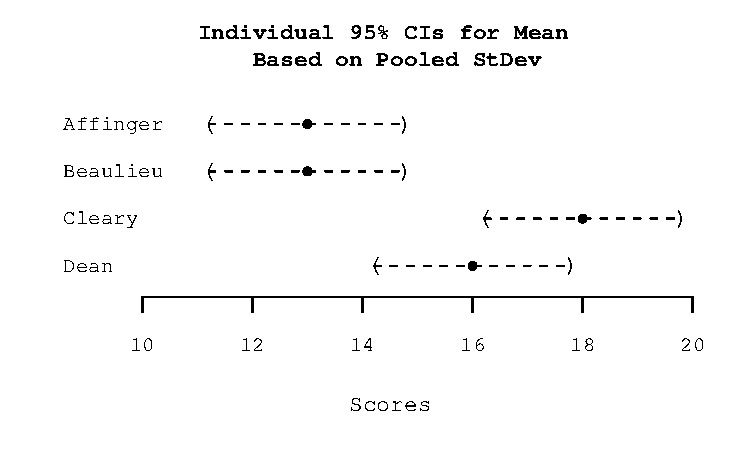
\includegraphics[width=3.5in]{includes/Item7_R.pdf}
\end{figure}

\renewcommand{\labelenumi}{\arabic{enumi}.}
\begin{enumerate}[leftmargin=1cm, itemsep=.2em]
\item Unfortunately, we are missing the ANOVA table from the output. Use the information given above to construct the ANOVA table and conduct a test (5\% level) for any significant differences among the average scores assigned by the four instructors.  Be sure to include hypotheses and a conclusion.   If you have trouble getting one part of the table that you need to complete the rest (or the next question), make a reasonable guess or ask for assistance (for a small point fee). 
\item After completing the ANOVA table, construct a 95\% confidence interval for the average score given by Dr. Affinger. \textit{Note: Your answer should be consistent with the graphical display.}
\end{enumerate}


\section{\textbf{Additional Examples of Good Assessment Items}}

\subsection{\textbf{\textit{Item 8}}}
Let Y denote the amount a student spends on textbooks for one semester. Suppose Nancy, who is statistically savvy, wants to know how fall, semester 1, and spring, semester 2, compare.  In particular, suppose she is interested in the averages ?1 and ?2.  You may assume that Nancy has taken several statistics courses and knows a lot about statistics, including how to interpret confidence intervals and hypothesis tests.  You have random samples from each semester and are to analyze the data and write a report.  You seek advice from four persons:

\begin{enumerate}[leftmargin=1cm, itemsep=.2em]
\item \textbf{Rudd says,} ``Conduct an $\alpha=.05$ test of $H_0: \mu_1=\mu_2$ vs. $H_A: \mu_1 \neq \mu_2$ and tell Nancy whether you reject $H_0$.''

\item \textbf{Linda says,} ``Report a 95\% confidence interval for $?_1 - ?_2$ .''


\item \textbf{Steve says,} ``Conduct a test of $H_0: \mu_1=\mu_2$ vs. $H_A: \mu_1 \neq \mu_2$ and report to Nancy the \textit{p}-value from the test.''

\item \textbf{Gloria says,} ``Compare $\bar{y}_1$  to $\bar{y}_2$.  If $\bar{y}_1 > \bar{y}_2$,  then test $H_0: \mu_1=\mu_2$ vs. $H_A: \mu_1 > \mu_2$ using $\alpha =.05$ and tell Nancy whether you reject $H_0$.  If $\bar{y}_1 < \bar{y}_2$,  then test $H_0: \mu_1=\mu_2$ vs. $H_A: \mu_1 < \mu_2$ using $\alpha = .05$ and tell Nancy whether you reject $H_0$.''
\end{enumerate}

Rank the four pieces of advice from worst to best and explain why you rank them as you do. That is, explain what makes one better than another.

\subsection{\textbf{\textit{Item 9}}}
Researchers took random samples of subjects from two populations and applied a Wilcoxon-Mann-Whitney test to the data; the \textit{P}-value for the test, using a nondirectional alternative, was .06.  For each of the following, say whether the statement is true or false and why.
\begin{enumerate}[leftmargin=1cm, itemsep=.2em]
\item There is a 6\% chance that the two population distributions really are the same.
\item If the two population distributions really are the same, then a difference between the two samples as extreme as the difference that these researchers observed would only happen 6\% of the time.
\item If a new study were done that compared the two populations, there is a 6\% probability that $H_0$ would be rejected again.
\item If $\alpha = .05$ and a directional alternative were used, and the data departed from $H_0$ in the direction specified by the alternative hypothesis, then $H_0$ would be rejected.
\end{enumerate}

\subsection{\textbf{\textit{Item 10}}}
An article on the CNN web page (\url{www.cnn.com/HEALTH/9612/16/faith.healing/index.html}) on Monday begins with the sentence, ``Family doctors overwhelmingly believe that religious faith can help patients heal, according to a survey released Monday.''  Later, the article states, ``Medical researchers say the benefits of religion may be as simple as helping the immune system by reducing stress,'' and Dr. Harold Koenig is reported to say that ``people who regularly attend church have half the rate of depression of infrequent churchgoers.''
  
Use the language of statistics to critique the statement by Dr. Koenig and the claim, suggested by the article, that religious faith and practice help people fight depression. You will want to select some of the following words in your critique: observational study, experiment, blind, double-blind, precision, bias, sample, spurious, confounding, causation, association, random, valid, reliable.

\subsection{\textbf{\textit{Item 11}}}
Francisco Franco (Class of '98) weighed 100 Hershey's Kisses (with almonds).  He found that the sample average was 4.80 grams and the SD was .28 grams. \textit{In the context of this setting,} explain what is meant by the sampling distribution of an average.

\subsection{\textbf{\textit{Item 12}}}
A gardener wishes to compare the yields of three types of pea seeds---type A, type B, and type C.  She randomly divides the type A seeds into three groups and plants some in the east part of her garden, some in the central part of the garden, and some in the west part of the garden.  Then, she does the same with the type B seeds and type C seeds.
\begin{enumerate}[leftmargin=1cm, itemsep=.2em]
\item \textit{What kind} of experimental design is the gardener using?
\item \textit{Why} is this kind of design used in this situation?  (Explain in the \textit{context of the situation.})
\end{enumerate}

\subsection{\textbf{\textit{Item 13}}}
The scatterplot shows how divorce rate, y, and marriage rate, x, are related for a collection of 10 countries.  The regression line has been added to the plot.

\begin{marginfigure}
\centering
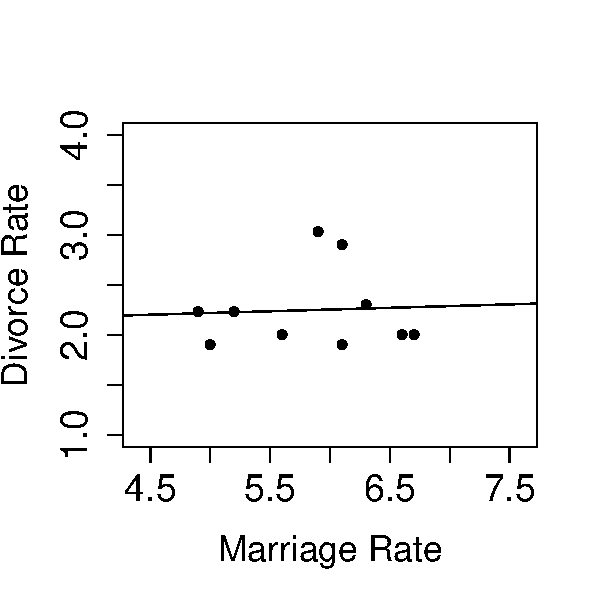
\includegraphics{includes/Item13_R.pdf}
\end{marginfigure}

\begin{enumerate}[leftmargin=1cm, itemsep=.2em]
\item The U.S. is not one of the 10 points in the original collection of countries.  It happens that the U.S. has a higher marriage rate than any of the 10 countries.  Moreover, the divorce rate for the U.S. is higher than one would expect, given the pattern of the other countries.  How would adding the U.S. to the data set affect the regression line?  Why?
\item Think about the scatterplot and regression line after the U.S. has been added to the data set.  Provide a sketch of the residual plot.  Label the axes and identify the U.S. on your plot with a triangle.
\end{enumerate}


\subsection{\textbf{\textit{Item 14}}}
Researchers wanted to compare two drugs, formoterol and salbutamol, in aerosol solution to a placebo for the treatment of patients who suffer from exercise-induced asthma.  Patients were to take a drug or the placebo, do some exercise, and then have their ``forced expiratory volume'' measured.  There were 30 subjects available. (Based on A.N. Tsoy, et al., \textit{European Respiratory Journal 3} (1990): 235; via Berry, \textit{Statistics: A Bayesian Perspective}.)
\begin{enumerate}[leftmargin=1cm, itemsep=.2em]
\item Should this be an experiment or an observational study?  Why?
\item Within the context of this setting, what is the placebo effect?
\item Briefly explain how to set up a randomized blocks design (RBD) here.
\item How would an RBD be helpful?  That is, what is the main advantage of using an RBD in a setting like this?
\end{enumerate}

\subsection{\textbf{\textit{Item 15}}}
I noticed that eight students from the 114 class attended the review session prior to the second exam (in April).  The average score among those eight students was lower than the average for the 21 students who did not attend the review session.  Suppose I want to use this information in a study of the effectiveness of review sessions.
\begin{enumerate}[leftmargin=1cm, itemsep=.2em]
\item What kind of study is this, observational or experimental?  Why?
\item What kind(s) of sampling error(s) or bias(es) might be of concern here?
\item (Hypothetical)  I gave the data for the eight who attended and for the 21 who did not attend to my friend George.  George used the data to conduct a hypothesis test.  Does a hypothesis test make sense?  If so, what is $H_0$?  If not, why not?
\end{enumerate}



\subsection{\textbf{\textit{Item 16}}}
For each of the following three settings, state the type of analysis you would conduct (e.g., one-sample \textit{t}-test, regression, chi-square test of independence, chi-square goodness-of-fit test, etc.) if you had all the raw data and specify the roles of the variable(s) on which you would perform the analysis, but \textit{do not actually carry out the analysis}.
\begin{enumerate}[leftmargin=1cm, itemsep=.2em]
\item Elizabeth Larntz (Class of '02) measured the effect of exercise on pulse for each of 13 students.  She measured pulse before and after exercise (doing 30 jumping jacks) and found that the average change was 55.1 and the SD of the changes was 18.4.  How would you analyze the data?
\item Three HIV treatments were tested for their effectiveness in preventing progression of HIV in children.  Of 276 children given drug A, 259 lived and 17 died. Of 281 children given drug B, 274 lived and seven died.  Of 274 children given drug C, 264 lived and 10 died.  How would you analyze the data?
\item A researcher was interested in the relationship between forearm length and height.  He measured the forearm lengths and heights of each of 16 women.  How would you analyze these data?
\end{enumerate}

\subsection{\textbf{\textit{Item 17}}}
I had Data Desk construct parallel dotplots of the data from four samples.  I then conducted a test of $H_0: \mu_1=\mu_2=\mu_3=\mu_4$ and rejected $H_0$ at the $\alpha = .05$ level.  I also tested $H_0: \mu_1=\mu_2=\mu_3$ and rejected $H_0$ at the $\alpha = .05$ level.  However, when I tested$H_0: \mu_2=\mu_3$ using $\alpha = .05$, I did \textit{not} reject $H_0$.  Likewise, when I tested $H_0: \mu_1=\mu_4$ using $\alpha = .05$, I did \textit{not} reject $H_0$.
\begin{enumerate}[leftmargin=1cm, itemsep=.2em]
\item Your job is to sketch a graph of the parallel dotplots of the data. That is, based on what I told you about the tests, you should have an idea of how the data look. Use that idea to draw a graph.  Indicate the sample means with triangles that you add to the dotplots.
\item It is possible to get data with the same sample means that you graphed in part 1, but for which the hypothesis $H_0: \mu_1=\mu_2=\mu_3=\mu_4$ is not rejected at the $\alpha = .05$ level.  Provide a graph of this situation.  That is, keep the same sample means (triangles) you had from part 1, but show how the data would have been different if $H_0$ were not to be rejected.
\end{enumerate}

\subsection{\textbf{\textit{Item 18}}}
Atley Chock (Class of `02) collected data on a random sample of 12 breakfast cereals.  He recorded x = fiber (in grams/ounce) and y = price (in cents/ounce).  A scatterplot of the data shows a linear relationship.  The fitted regression model is

\begin{equation*}
\hat{y} = 17.42 + 0.62x
\end{equation*}
  
The sample correlation coefficient, $r$, is 0.23.  The SE of $b_1$ is .81.   Also, $s_{y|x}$ = 3.1.
\begin{enumerate}[leftmargin=1cm, itemsep=.2em]
\item Find $r^2$ and interpret $r^2$ in the context of this problem.
\item Suppose a cereal has 2.63 grams of fiber/ounce and costs 17.3 cents/ounce.  What is the residual for this cereal?
\item Interpret the value of $s_{y|x}$ in the context of this problem.  That is, what does it mean to say that $s_{y|x}$ = 3.1?
\item In the context of this problem, explain what is meant by ``the regression effect.''
\end{enumerate}

\subsection{\textbf{\textit{Item 19}}}
Give a rough estimate of the sample correlation for the data in each of the scatterplots below.

\begin{figure}[ht]
\centering
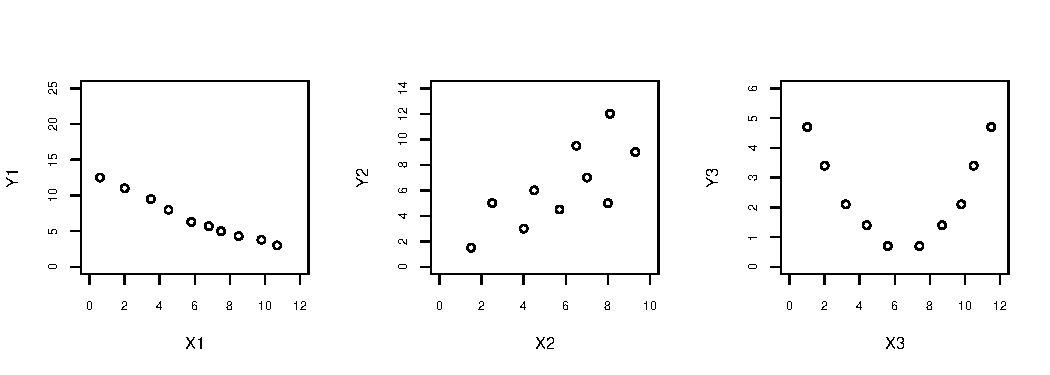
\includegraphics[width=6.5in]{includes/Item19_R.pdf}
\end{figure}


\subsection{\textbf{\textit{Item 20}}}
A matched pairs experiment compares the taste a regular cheese pizza of Pizza Joe's to Domino's.  Each subject tastes two unmarked pieces of pizza, one of each type, in random order and states which he or she prefers.  Of the 50 subjects who participate in the study, 21 prefer Pizza Joe's.   
\begin{enumerate}[leftmargin=1cm, itemsep=.2em]
\item Find a 96\% confidence interval for the proportion of the population that prefers Pizza Joe's to Domino's.
\item How large a sample is required if the desired margin of error of the confidence interval is 4\%?
\end{enumerate}

\subsection{\textbf{\textit{Item 21}}}
It was claimed that 1 out of 5 cardiologists takes an aspirin a day to prevent hardening of the arteries.  Suppose the claim is true.  If 1,500 cardiologists are selected at random, what is the probability that at least 275 of the 1,500 take an aspirin a day? 

\subsection{\textbf{\textit{Item 22}}}
Identify whether a scatterplot would or would not be an appropriate visual summary of the relationship between the variables.  In each case, explain your reasoning.  
\begin{enumerate}[leftmargin=1cm, itemsep=.2em]
\item Blood pressure and age
\item Region of country and opinion about stronger gun control laws
\item Verbal SAT and math SAT score
\item Handspan and gender (male or female)
\end{enumerate}

\subsection{\textbf{\textit{Item 23}}}
The paragraphs that follow each describe a situation that calls for some type of statistical analysis.  For each, you should:
\renewcommand{\labelenumi}{\arabic{enumi}.}
\begin{enumerate}[leftmargin=1cm, itemsep=.2em]
\item Give the name of an appropriate statistical procedure to apply (from the list below). You may use the same procedure more than once, and some questions might have more than one correct answer.
\item In some problems, you will also be given a \textit{p}-value. Use it to reach a conclusion for that specific problem.  Be sure to say something more than just Reject $H_0$ or Fail to Reject $H_0$. (Assume a 5\% significance level.) 
\end{enumerate}

Some statistical procedures you might choose:
\begin{table}[!ht]
\begin{center}
\begin{tabular}{ll}
\hline
Confidence interval (for a mean, p, \ldots) & Normal distribution\\
Determining sample size	& Correlation\\
Test for a mean	 & Simple linear regression\\
Test for proportion & Multiple regression\\
Difference in means (paired data) & Two-way table (chi-square test)\\
Difference in means (two independent samples) & ANOVA for difference in means\\
Difference in proportions & Two-way ANOVA for means\\
\hline
\end{tabular}
\end{center}
\end{table}

\renewcommand{\labelenumi}{\Alph{enumi}.}

\begin{enumerate}[leftmargin=1cm, itemsep=.2em]
\item Anthropologists have found two burial mounds in the same region. They know several tribes lived in the region and that the tribes have been classified according to different lengths of skulls. They measure a random sample of skulls found in each burial mound and wish to determine if the two mounds were made by different tribes.  (\textit{p}-value = 0.0082) 

\bigskip
	
\item The Hawaiian Planters Association is developing three new strains of pineapple (call them A, B, and C) to yield pulp with higher sugar content. Twenty plants of each variety (60 plants in all) are randomly distributed into a two-acre field. After harvesting, the resulting pineapples are measured for sugar content and the yields are recorded for each strain.  Are there significant differences in average sugar content between the three strains? (\textit{p}-value = 0.987)
\bigskip	
\item Researchers were commissioned by the Violence In Children's Television Investigative Monitors (VICTIM) to study the frequency of depictions of violent acts in Saturday morning TV fare.  They selected a random sample of 40 shows that aired during this time period over a 12-week period.  Suppose 28 of the 40 shows in the sample were judged to contain scenes depicting overtly violent acts.  How should they use this information to make a statement about the population of all Saturday morning TV shows?
\bigskip	
\item The Career Planning Office is interested in seniors' plans and how they might relate to their majors.  A large number of students are surveyed and classified according to their MAJOR (Natural Science, Social Science, Humanities) and FUTURE plans (Graduate School, Job, Undecided).  Are the type of major and future plans related?  (\textit{p}-value = 0.047)
\bigskip
\item \textit{Sophomore Magazine} asked a random sample of 15 year olds if they were sexually active (yes or no).  They would like to see if there is a difference in the responses between boys and girls.     (\textit{p}-value = 0.029)
\bigskip	
\item Every week during the Vietnam War, a body count (number of enemy killed) was reported by each army unit. The last digits of these numbers should be fairly random.  However, suspicions arose that the counts might have been fabricated.  To test this, a large random sample of body count figures was examined and the frequency with which the last digit was a 0 or a 5 was recorded.  Psychologists have shown that people making up their own random numbers will use these digits less often than random chance would suggest (i.e., 103 sounds like a more ``real" count than 100).  If the data were authentic counts, the proportion of numbers ending in 0 or 5 should be about 0.20.  (\textit{p}-value=0.002)
\bigskip	
\item In one of his adventures, Sherlock Holmes found footprints made by the criminal at the scene of a crime and measured the distance between them. After sampling many people, measuring their height and length of stride, he confidently announced that he could predict the height of the suspect. How?
\end{enumerate}


\subsection{\textbf{\textit{Item 24}}}
How accurate are radon detectors of a type sold to homeowners?  To answer this question, university researchers placed 12 detectors in a chamber that exposed them to 105 picocuries per liter of radon.  The detector readings found are below.  A printout of the descriptive statistics from Minitab follows. 

\begin{table}[!ht]
\begin{center}
\begin{tabular}{llllll}
91.9	& 97.8 & 111.4 & 122.3 & 105.4 & 95.0\\
103.8 & 99.6 & 96.6 & 119.3 & 104.8 & 101.7\\
\end{tabular}
\end{center}
\end{table}

\begin{table}[!ht]
\begin{center}
\begin{tabular}{lllllllllll}
\texttt{Variable} & \texttt{N} & \texttt{Mean} & \texttt{Median} &    \texttt{TrMean} & \texttt{StDev} & \texttt{SE Mean} & \texttt{Minimum}  & \texttt{Maximum}      &   \texttt{Q1}   &      \texttt{Q3}\\
\texttt{readings} & \texttt{12} & \texttt{104.13} & \texttt{102.75} & \texttt{103.54} & \texttt{9.40} & \texttt{2.71} &      \texttt{91.90}  &  \texttt{122.30}   &   \texttt{96.90}   &  \texttt{109.90}\\
\end{tabular}
\end{center}
\end{table}

\renewcommand{\labelenumi}{\arabic{enumi}.}

\begin{enumerate}[leftmargin=1cm, itemsep=.2em]
\item Is there convincing evidence that the mean 20 readings of all detectors of this type differs from the true value of 105?  Perform the appropriate hypothesis test with $\alpha  = .05$.
\item What is the Type I error associated with this problem?
\item What is the Type II error associated with this problem?
\item What is the probability of a type II error if the reading of the detectors is too low by 5 picocuries (really 100 when it should read 105)?
\end{enumerate}


\subsection{\textbf{\textit{Item 25}}}
According a U.S. Food and Drug Administration (FDA) study, a cup of coffee contains an average of 115 mg of caffeine, with the amount per cup ranging from 60 to 180 mg depending on the brewing method.  Suppose you want to repeat the FDA experiment to obtain an estimate of the mean caffeine content to within 5 mg with 95\% using your favorite brewing method.  In problems such as this, we can estimate the standard deviation of the population to be $\frac{1}{4}$ of the range. How many cups of coffee must you brew?  

\subsection{\textbf{\textit{Item 26}}}
An advertisement claims that by applying a particular drug, hair is restored to bald-headed men.  Outline the design of an experiment you would use to examine this claim.  Assume you have money to use 20 bald men in this experiment.  

\subsection{\textbf{\textit{Item 27}}}
A study of iron deficiency among infants compared samples of infants following different feeding regimens.  One group contained breast-fed infants, while the children in another group were fed a standard baby formula without any iron supplements.  Here are the summary results on blood hemoglobin levels at 12 months of age:

\begin{table}[!ht]
\begin{center}
\begin{tabular}{llll}
\hline
Group & N & $\bar{X}$ & s\\
\hline
Breast-fed	 & 23 & 13.3 & 1.7\\
Formula & 19 & 12.4 & 1.8\\
\hline
\end{tabular}
\end{center}
\end{table}

Assume that the blood hemoglobin levels in children (both breast-fed and formula-fed) are normally distributed.  Do a significance test to determine the statistical significance of the observed difference.

\subsection{\textbf{\textit{Item 28}}}
Which implies a stronger linear relationship, a correlation of $+0.4$ or a correlation of $-0.6$?  Briefly explain your choice.

\subsection{\textbf{\textit{Item 29}}}
A group of physicians subjected the polygraph to the same careful testing given to medical diagnostic tests.  They found that if 1,000 people were subjected to the polygraph and 500 told the truth and 500 lied, the polygraph would indicate that approximately 185 of the truth-tellers were liars and 120 of the liars were truth-tellers.  In the application of the polygraph test, an individual is presumed to be a truth-teller until indicated that s/he is a liar. What is a type I error in the context of this problem?  What is the probability of a type I error in the context of this problem?  What is a type II error in the context of this problem?  What is the probability of a type II error in the context of this problem?


\subsection{\textbf{\textit{Item 30}}}
Audiologists recently developed a rehabilitation program for hearing-impaired patients in a Canadian program for senior citizens.  A simple random sample of the 30 residents of a particular senior citizens home and the seniors were diagnosed for degree and type of sensorineural hearing loss which was coded as follows: 1 = hear within normal limits, 2 = high-frequency hearing loss, 3 = mild loss, 4 = mild-to-moderate loss, 5 = moderate loss, 6 = moderate-to-severe loss, and 7 = severe-to-profound loss.  The data are as follows: 

\begin{table}[!ht]
\begin{center}
\begin{tabular}{lllllllllllllll}
6 & 7 & 1 & 1 & 2 & 6 & 4 & 6 & 4 & 2 & 5 & 2 & 5 & 1&  5\\
4 & 6 & 6 & 5 & 5 & 5 & 2 & 5 & 3 & 6 & 4 & 6 & 6 & 4 & 2\\
\end{tabular}
\end{center}
\end{table}
 
\begin{enumerate}[leftmargin=1cm, itemsep=.2em]
\item Create a boxplot of the data.
\item Give a good description of the data.
\item Find a 95\% confidence interval for the mean hearing loss of senior citizens in this Canadian program.   The mean and standard deviation of the above data are 4.2 and 1.808, respectively. Interpret the interval.
\end{enumerate}

\subsection{\textbf{\textit{Item 31}}}
A utility company was interested in knowing if agricultural customers would use less electricity during peak hours if their rates were different during those hours.  Customers were randomly assigned to continue to get standard rates or to receive the time-of-day structure.  Special meters were attached that recorded usage during peak and off-peak hours; the technician who read the meter did not know what rate structure each customer had.
\begin{enumerate}[leftmargin=1cm, itemsep=.2em]
\item Is this an observation study or experiment?  Defend your answer.
\item What is the explanatory and response variable?
\item List a potential confounding variable in this work.
\item Is this a matched-pair design?  Defend your answer.
\end{enumerate}


\subsection{\textbf{\textit{Item 32}}}
At the beginning of the semester, we measured the width of a page in our statistics book.  Below is the scatterplot of the first measurement vs. the second measurement. 

\begin{marginfigure}
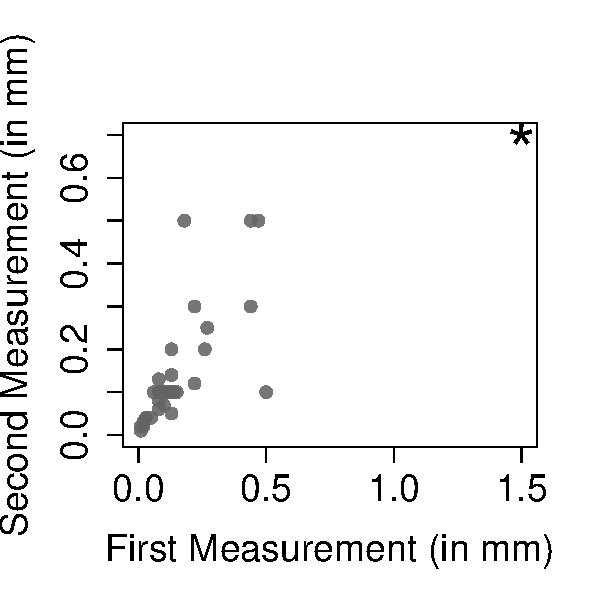
\includegraphics{includes/Item32_R.pdf}
\end{marginfigure}
 
\begin{enumerate}[leftmargin=1cm, itemsep=.2em]
\item Describe the distribution.
\item Estimate the correlation with and without the starred point.
\end{enumerate}

\subsection{\textbf{\textit{Item 33}}}
A study in the \textit{Journal of Leisure Research} investigated the relationship between academic performance and leisure activities.  Each in a sample of 159 high-school students was asked to state how many leisure activities they participated in weekly.  From the list, activities that involved reading, writing, or arithmetic were labeled ``academic leisure activities.'' Some of the results are in the table below:

\begin{table}[!ht]
\begin{center}
\begin{tabular}{lrr}
\hline
& Mean & Standard Deviation\\
\hline
GPA & 2.96 & 0.71\\
Number of leisure activities & 12.38 & 5.07\\
Number of academic leisure activities & 2.77 & 1.97\\
\hline
\end{tabular}
\end{center}
\end{table}

Based on these numbers (and knowing that the GPA is a value between 0 and 4 and the number of activities cannot be negative), discuss the potential skewness of each of the above variables.

\subsection{\textbf{\textit{Item 34}}}
Events A and B are disjoint.  Discuss whether or not A and B can be independent. 

\subsection{\textbf{\textit{Item 35}}}
A sample of 200 mothers and a sample of 200 fathers were taken.  The age of the mother when she had her first child and the age of the father when he had his first child were recorded.

\begin{enumerate}[leftmargin=1cm, itemsep=.2em]
\item Describe the data for the mothers' age.
\item Describe the data for the fathers' age.
\begin{marginfigure}
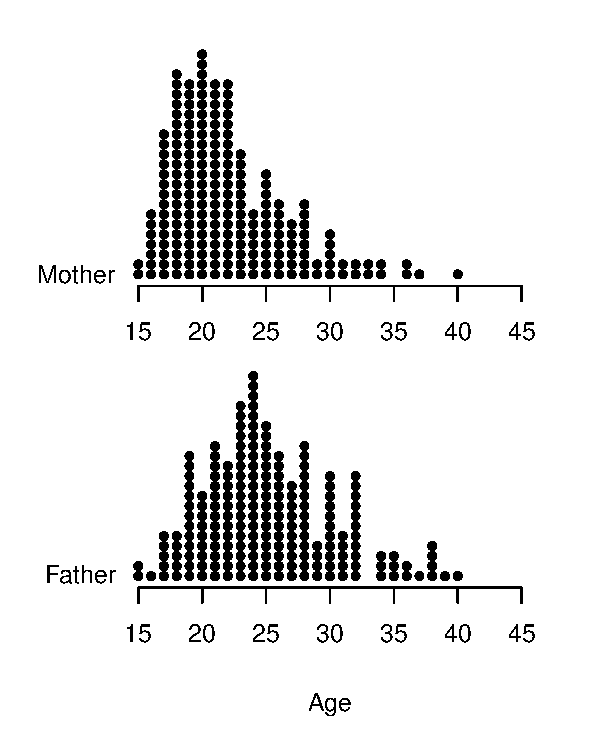
\includegraphics[width=2.75in]{includes/Item35.pdf}
\end{marginfigure}
\item Compare the distributions.
\item A suggestion is made to check the correlation between the ages if we wish to compare the two populations.  Is this a good suggestion?  Why or why not?
\end{enumerate}

\added{\subsection{\textbf{\textit{Item 36}}}
When doing a randomized experiment, the original randomization of units to
treatment groups breaks the association between
\begin{enumerate} [leftmargin=2cm, itemsep=.2em]
\item The explanatory variable and the response variable
\item The explanatory variable and confounding variables
\item The response variable and confounding variables
\end{enumerate}}

\added{\subsection{\textbf{\textit{Item 37}}}
When doing a randomization test, the simulated re-randomization of units to
treatment groups breaks the association between
\begin{enumerate} [leftmargin=2cm, itemsep=.2em]
\item The explanatory variable and the response variable
\item The explanatory variable and confounding variables
\item The response variable and confounding variables
\end{enumerate}}

\chapter{Appendix C: Example of Using Technology}
\vspace{-.53in}
   \noindent\color{graylight}\rule[0cm]{3.25in}{0.03cm} \\
    \noindent\color{graylight}\rule[0.4cm]{3.25in}{0.03cm} \\
\color{black}
%\vspace{-.25in}

\noindent\smallcaps{This example starts with a real-world situation, has students do a physical simulation using cards, and then brings in computer technology to automate the simulation. }

\section{\textbf{A Technology-Based Simulation to Examine the Effectiveness of Treatments for Cocaine Addiction}}
A study on the treatment of cocaine addiction described the results of an experiment comparing two drugs for helping addicts stay off cocaine (D.M. Barnes, ``Breaking the Cycle of Cocaine Addiction'', \textit{Science}, Vol. 241, 1988,  pp. 1029-1030).  A group of 48 cocaine addicts who were seeking treatment were randomly divided into two groups of 24.  One group was treated with a new drug called desipramine, while the other group was given lithium.  The results are summarized in the table below, where we consider patients who do not relapse as successfully treated. 

\begin{table}[!ht]
\begin{center}
\begin{tabular}{|l|c|c|}
\hline
& No Relapse & Relapse\\
\hline
Desipramine & 14 &  10\\
\hline
Lithium & 6 & 18\\
\hline
\end{tabular}
\end{center}
\end{table}

While we observe that desipramine was more successful than lithium in this particular experiment, can we conclude that the improvement is statistically significant. (i.e., Would we expect to see such a large difference if the drugs were equally effective and it was just the random assignment process that happened to get so many more successful cases in the desipramine group?)  We will address this question through simulation, first using a physical demonstration based on shuffling cards, then with a computer simulation that allows us to see the differences for many random assignments of the addicts to the treatment groups. \\
\vspace{12pt}
\newpage

\noindent\textbf{\textit{Physical Simulation}}\\
\vspace{3pt}
Take a deck of 54 playing cards (including two jokers) and remove six of the black cards (spades or clubs).  The remaining deck should match the subjects in the cocaine experiment with all the red cards and the jokers representing patients who relapsed and the 20 black cards representing patients who were treated successfully.  If we shuffle the deck and deal out two piles of 24 cards each, we will simulate the assignment of addicts to the two treatment groups when the success does not depend on which drug they take. Do so and fill in the two-way table with the ``success'' (black cards) and ``relapse'' (red/jokers) counts for each group.

\begin{table}[!ht]
\begin{center}
\begin{tabular}{|l|c|c|}
\hline
& No Relapse & Relapse\\
\hline
Desipramine &  &  \\
\hline
Lithium &  & \\
\hline
\end{tabular}
\end{center}
\end{table}

Note that once you know one number in the table, you can fill in the rest, as you know there are 24 in each treatment group and 20 will not relapse while 28 will relapse (that is why we sometimes say there is just one degree of freedom in the 2x2 table).  To keep things simple then, we can just keep track of one count, such as the number of ``no relapse'' in the desipramine group. 

Shuffle all the cards again, deal 24 for the desipramine group, and count the number of black cards. 

\begin{center}
Number of ``no relapse'' in desipramine group = \underline{\hspace{.5in}}
\end{center}

Pool the results for your class (counting \# of black cards in each random group of 24 cards assigned to the ``desipramine'' group) in a dotplot.  How often was the number of black cards as large as (or larger than) the 14 cases observed in the actual experiment? 

The \textit{p}-value of the original data is the proportion, assuming both drugs are equally effective, of random assignments that have 14 or more ``no relapse'' cases going to the desipramine group.  Estimate this proportion using the data in your class dotplot. \\
\vspace{12pt}

\noindent\textbf{\textit{Computer Simulation}}\\
\vspace{3pt}
To get a more accurate estimate of the proportion of random assignments that put 14 or more no relapse cases into the desipramine group, we'll turn to a computer simulation. 

Start with a data set (provided online) consisting of two columns and 48 rows.  The first column (Treatment) has the value ``desipramine'' in the first 24 rows and ``lithium'' in the remaining 24 rows.  The second column (Result) has the values ``no relapse'' and ``relapse'' to match the data in the original 2x2 table from the cocaine experiment. 

Have the computer permute the values in the ``Result'' column to represent a new random assignment of subjects to the treatment groups where the outcome does not depend on which drug was taken.  Count the number of ``no relapse'' cases in the desipramine treatment group and have the result stored somewhere.   Automate this process to repeat 1,000 times\footnote{\textit{Some technology alternatives:} The most difficult step here is to automate the simulations to record the counts for many random assignments.  Some packages, such as Fathom, have easy-to-use tools designed for exactly such purposes.  Others, such as Minitab, allow a bit of programming through macros that can be built in advance and repeated in a loop.  A somewhat less enlightening simulation could be accomplished with a stat package that allows generation of random data from a hypergeometric distribution, although students would then lose the connection to the physical randomizations.  Finally, an ambitious instructor could construct (or possibly find on the web) an applet to perform the required simulations and collect the results.}. 

Look at a histogram or dotplot of the distribution of counts for the 1,000 simulations.  Does it seem unusual to have as many as 14 ``no relapse'' cases in the desipramine group? 

Count the number of simulations that have 14 or more successes in the desipramine group (either from the graph, if feasible, or by sorting the simulated counts column) and divide by 1,000 to get another approximation of the \textit{p}-value for the original data.  

Does it seem reasonable that the larger number (14) of successful cases appeared in the desipramine group by chance, or would it be more appropriate to conclude that desipramine probably works better than lithium at treating cocaine addiction? 

%\chapter{Appendix D: Examples of Naked, Realistic, and Real Data}
\vspace{-.53in}
   \noindent\color{graylight}\rule[0cm]{3.25in}{0.03cm} \\
    \noindent\color{graylight}\rule[0.4cm]{3.25in}{0.03cm} \\
\color{black}
\vspace{-.25in}

\section{\textbf{Naked Data (not recommended)}}

Find the least squares \marginnote{\textit{Critique: Made-up data with no context (not recommended). The problem is purely computational with no possibility of meaningful interpretation.}} line for the data below.  Use it to predict Y when X=5.

\begin{table}[!ht]
\begin{center}
\begin{tabular}{|l|l|l|l|l|l|l|}
\hline
X & 1 & 2 & 3 & 4 & 6 & 8\\
\hline
Y & 3 & 4 & 6 & 7 & 14 & 20\\
\hline
\end{tabular}
\end{center}
\end{table}



\section{\textbf{Realistic Data (better, but still not the best)}}

The data below show\marginnote{\textit{Critique: A context has been added that makes the exercise more appealing and shows students a practical use of statistics.}} the number of customers in each of six tables at a restaurant and the size of the tip left at each table at the end of the meal.  Use the data to find a least squares line for predicting the size of the tip from the number of diners at the table.  Use your result to predict the size of the tip at a table that has five diners. 

\begin{table}[!ht]
\begin{center}
\begin{tabular}{|l|c|c|c|c|c|c|}
\hline
Diners & 1 & 2 & 3 & 4 & 6 & 8\\
\hline
Tip & \$3 & \$4 & \$6 & \$7 & \$14 & \$20\\
\hline
\end{tabular}
\end{center}
\end{table}


\newpage
\section{\textbf{Real Data (recommended)}}

The data below\marginnote{\textit{Critique: Data are from a real situation that should be of interest to students taking the course.}}  show the quiz scores (out of 20) and the grades on the midterm exam (out of 100) for a sample of eight students who took this course last semester.  Use these data to find a least squares line for predicting the midterm score from the quiz score. 
Assuming the quiz and midterm are of equal difficulty this semester and the same linear relationship applies this year, what is the predicted grade on the midterm for a student who got a score of 17 on the quiz? 

\begin{table}[!ht]
\begin{center}
\begin{tabular}{|l|l|l|l|l|l|l|l|l|}
\hline
Quiz & 20 & 15 & 13 & 18 & 18 & 20 & 14 & 16\\
\hline
Midterm & 92 & 72 & 72 & 95 & 88 & 98 & 65 & 77\\
\hline
\end{tabular}
\end{center}
\end{table}


\input{appendix-multivariate.tex}


%%
% The back matter contains appendices, bibliographies, indices, glossaries, etc.







\backmatter

\nobibliography{GAISE}
\bibliographystyle{plainnat}


\printindex

\end{document}

